\documentclass[../../compsys.tex]{subfiles}
\begin{document}

\chapter{Lecture 01: Introduction}

In this lecture we explore the journey of a YouTube video—from its storage as a file to its transformation into bytes, its transmission over networks, and finally, its display on your device. We will introduce key concepts such as processes, threads, distributed applications, system calls, and the role of the operating system in managing hardware resources.
\vfill
%%%%%%%%%%%%%%%%%%%%%%%%%%%%%%%%%%%%%%%%%%%%%%%%%%%%%%%%%%%%%%%%%%%%%%
\section{The Journey of a YouTube Video}
To illustrate these ideas, consider the journey of a YouTube video. The video begins its existence as a file stored on a storage device, is loaded into memory as bytes, transmitted as packets over the Internet, and finally rendered on your screen.

\begin{center}
  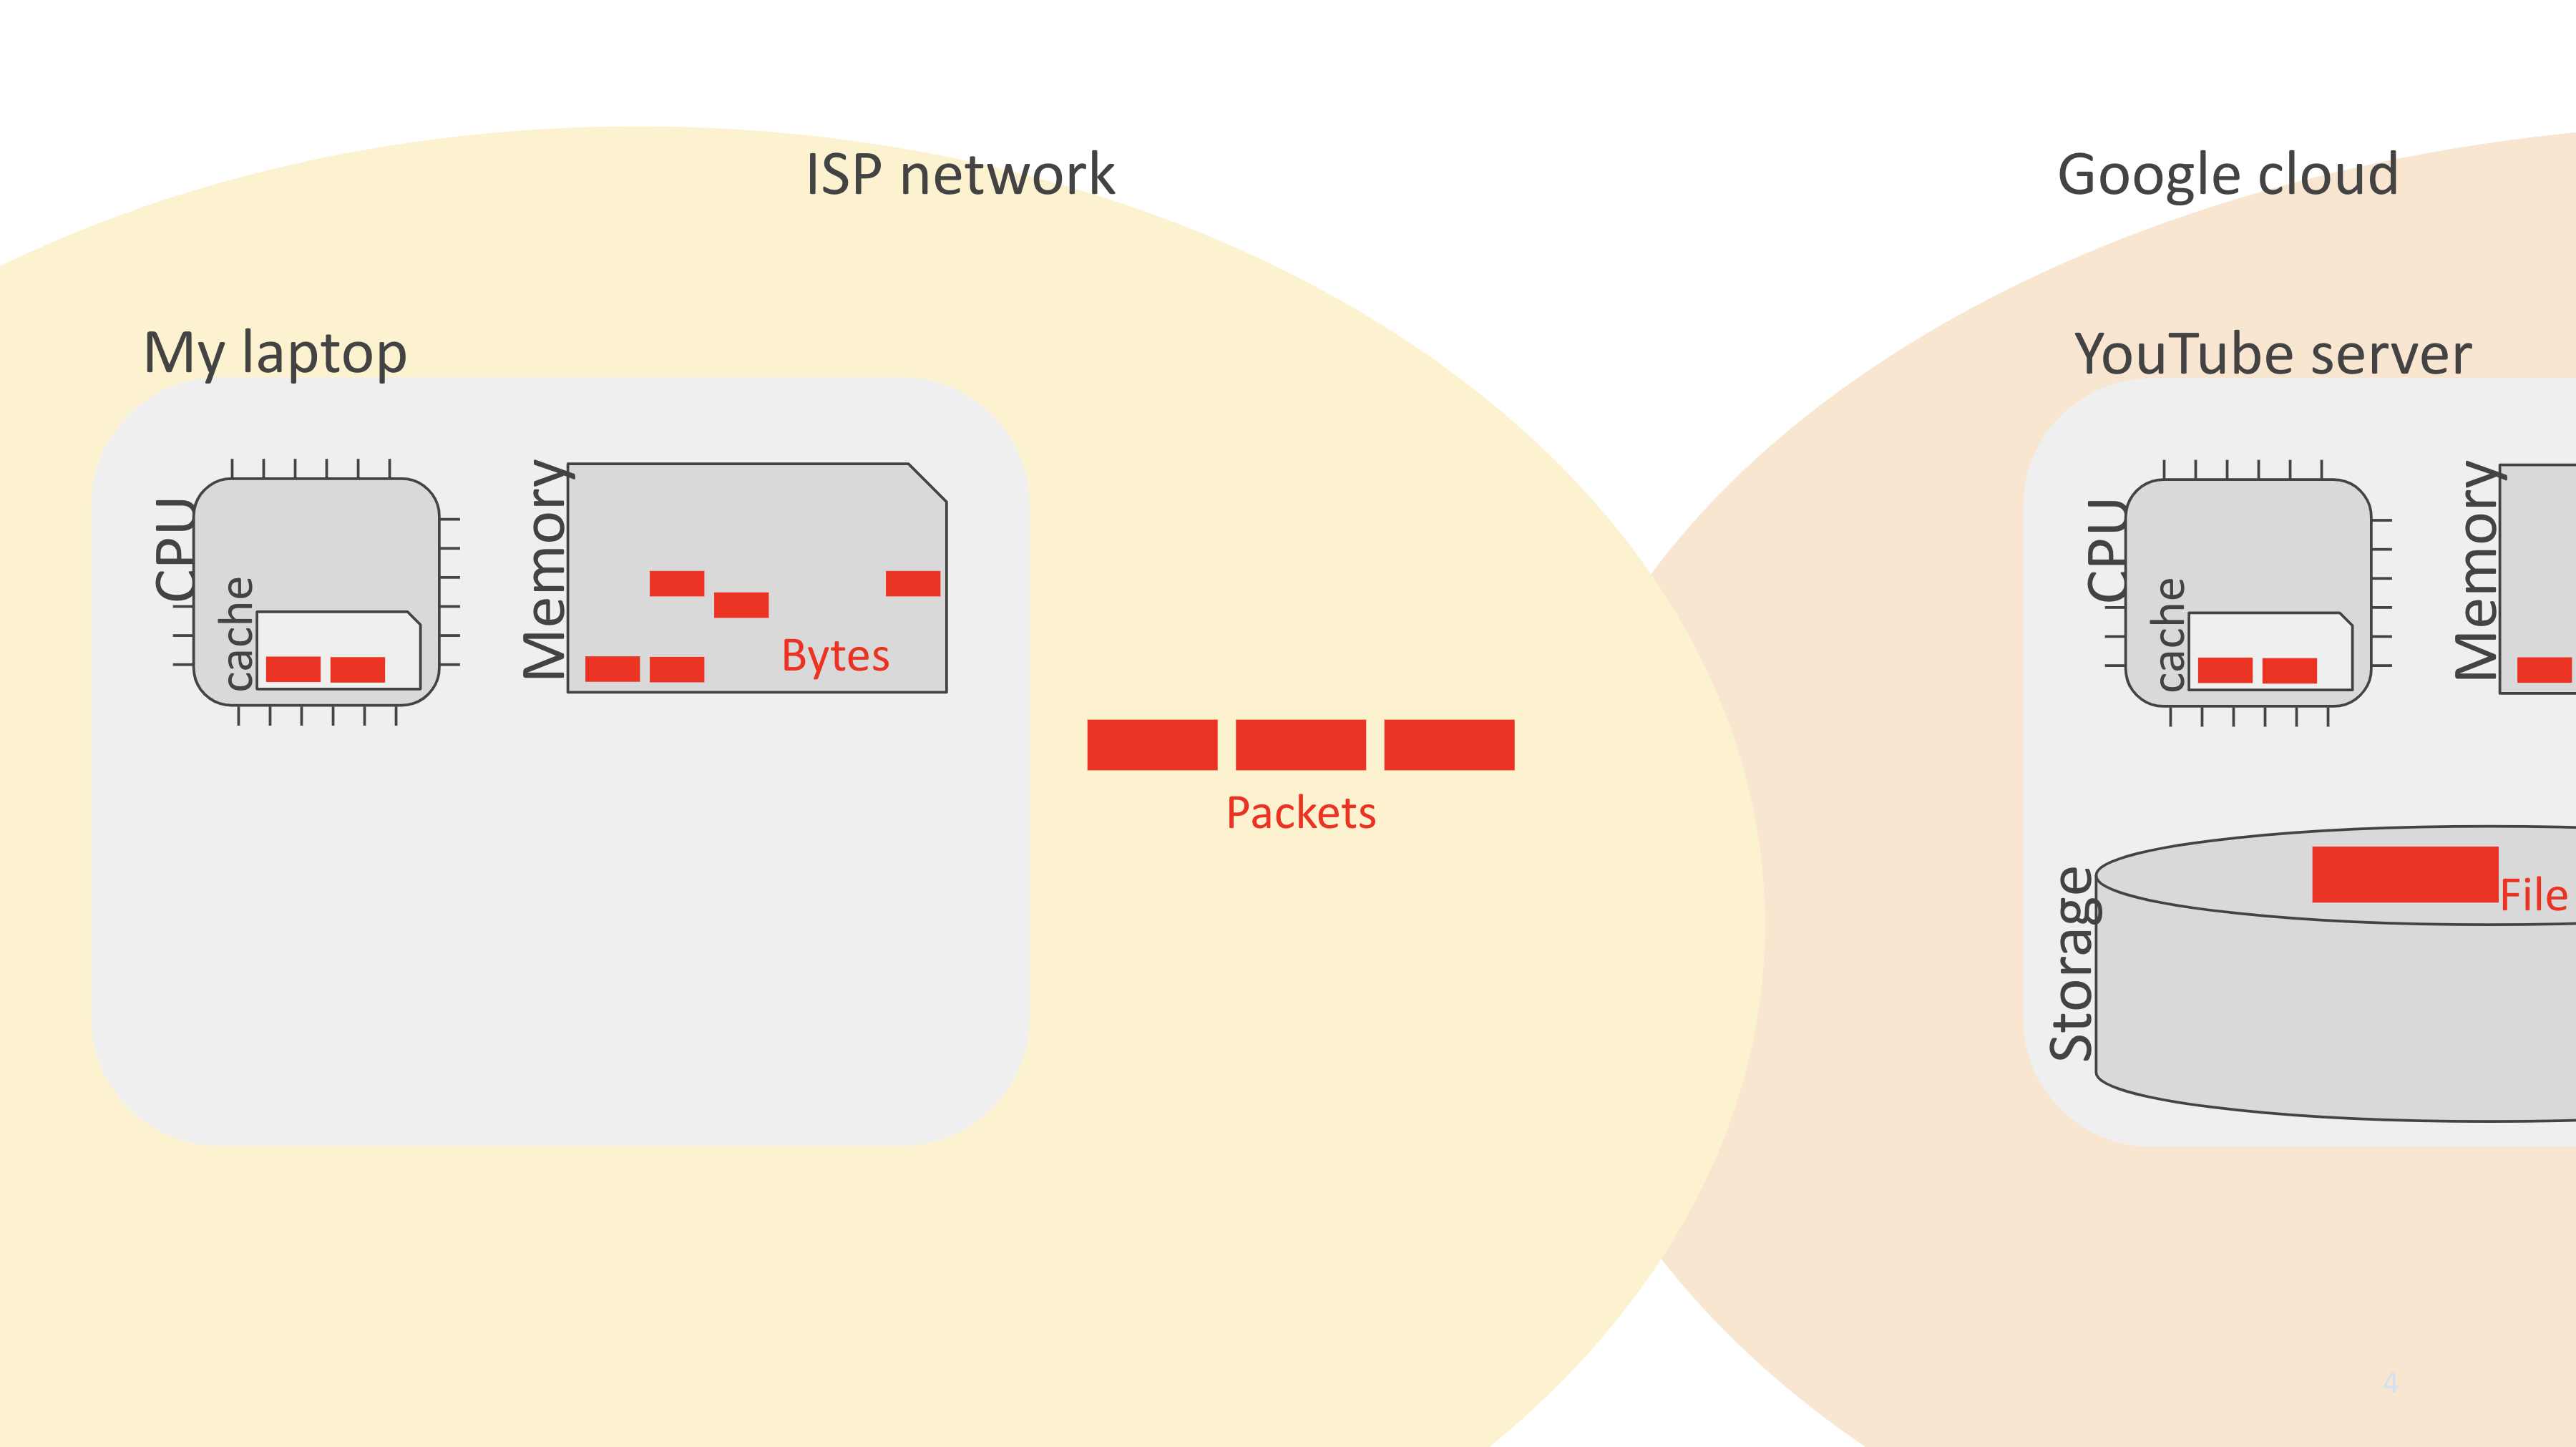
\includegraphics[width=0.85\textwidth]{chapters/L1/images/youtube.png}
\end{center}
\newpage
%%%%%%%%%%%%%%%%%%%%%%%%%%%%%%%%%%%%%%%%%%%%%%%%%%%%%%%%%%%%%%%%%%%%%%
\subsection{Start of the Journey: Inside the Laptop}
The journey begins on your laptop.\\[5px] 
\begin{minipage}{0.45\textwidth}
  \begin{justify}
    A computer hosts many different programs (e.g., a web browser, a ping utility, a git client). These programs, stored as files on disk, are invoked by user actions such as clicking an icon or typing a command. When a program is invoked, the computer creates a new \emph{process} in main memory. A process represents a running instance of a program and may consist of one or more \emph{threads}—individual units of execution within the process.
  \end{justify}
\end{minipage}
\hfill
\vline
\hfill
\begin{minipage}{0.45\textwidth}
  \begin{center}
  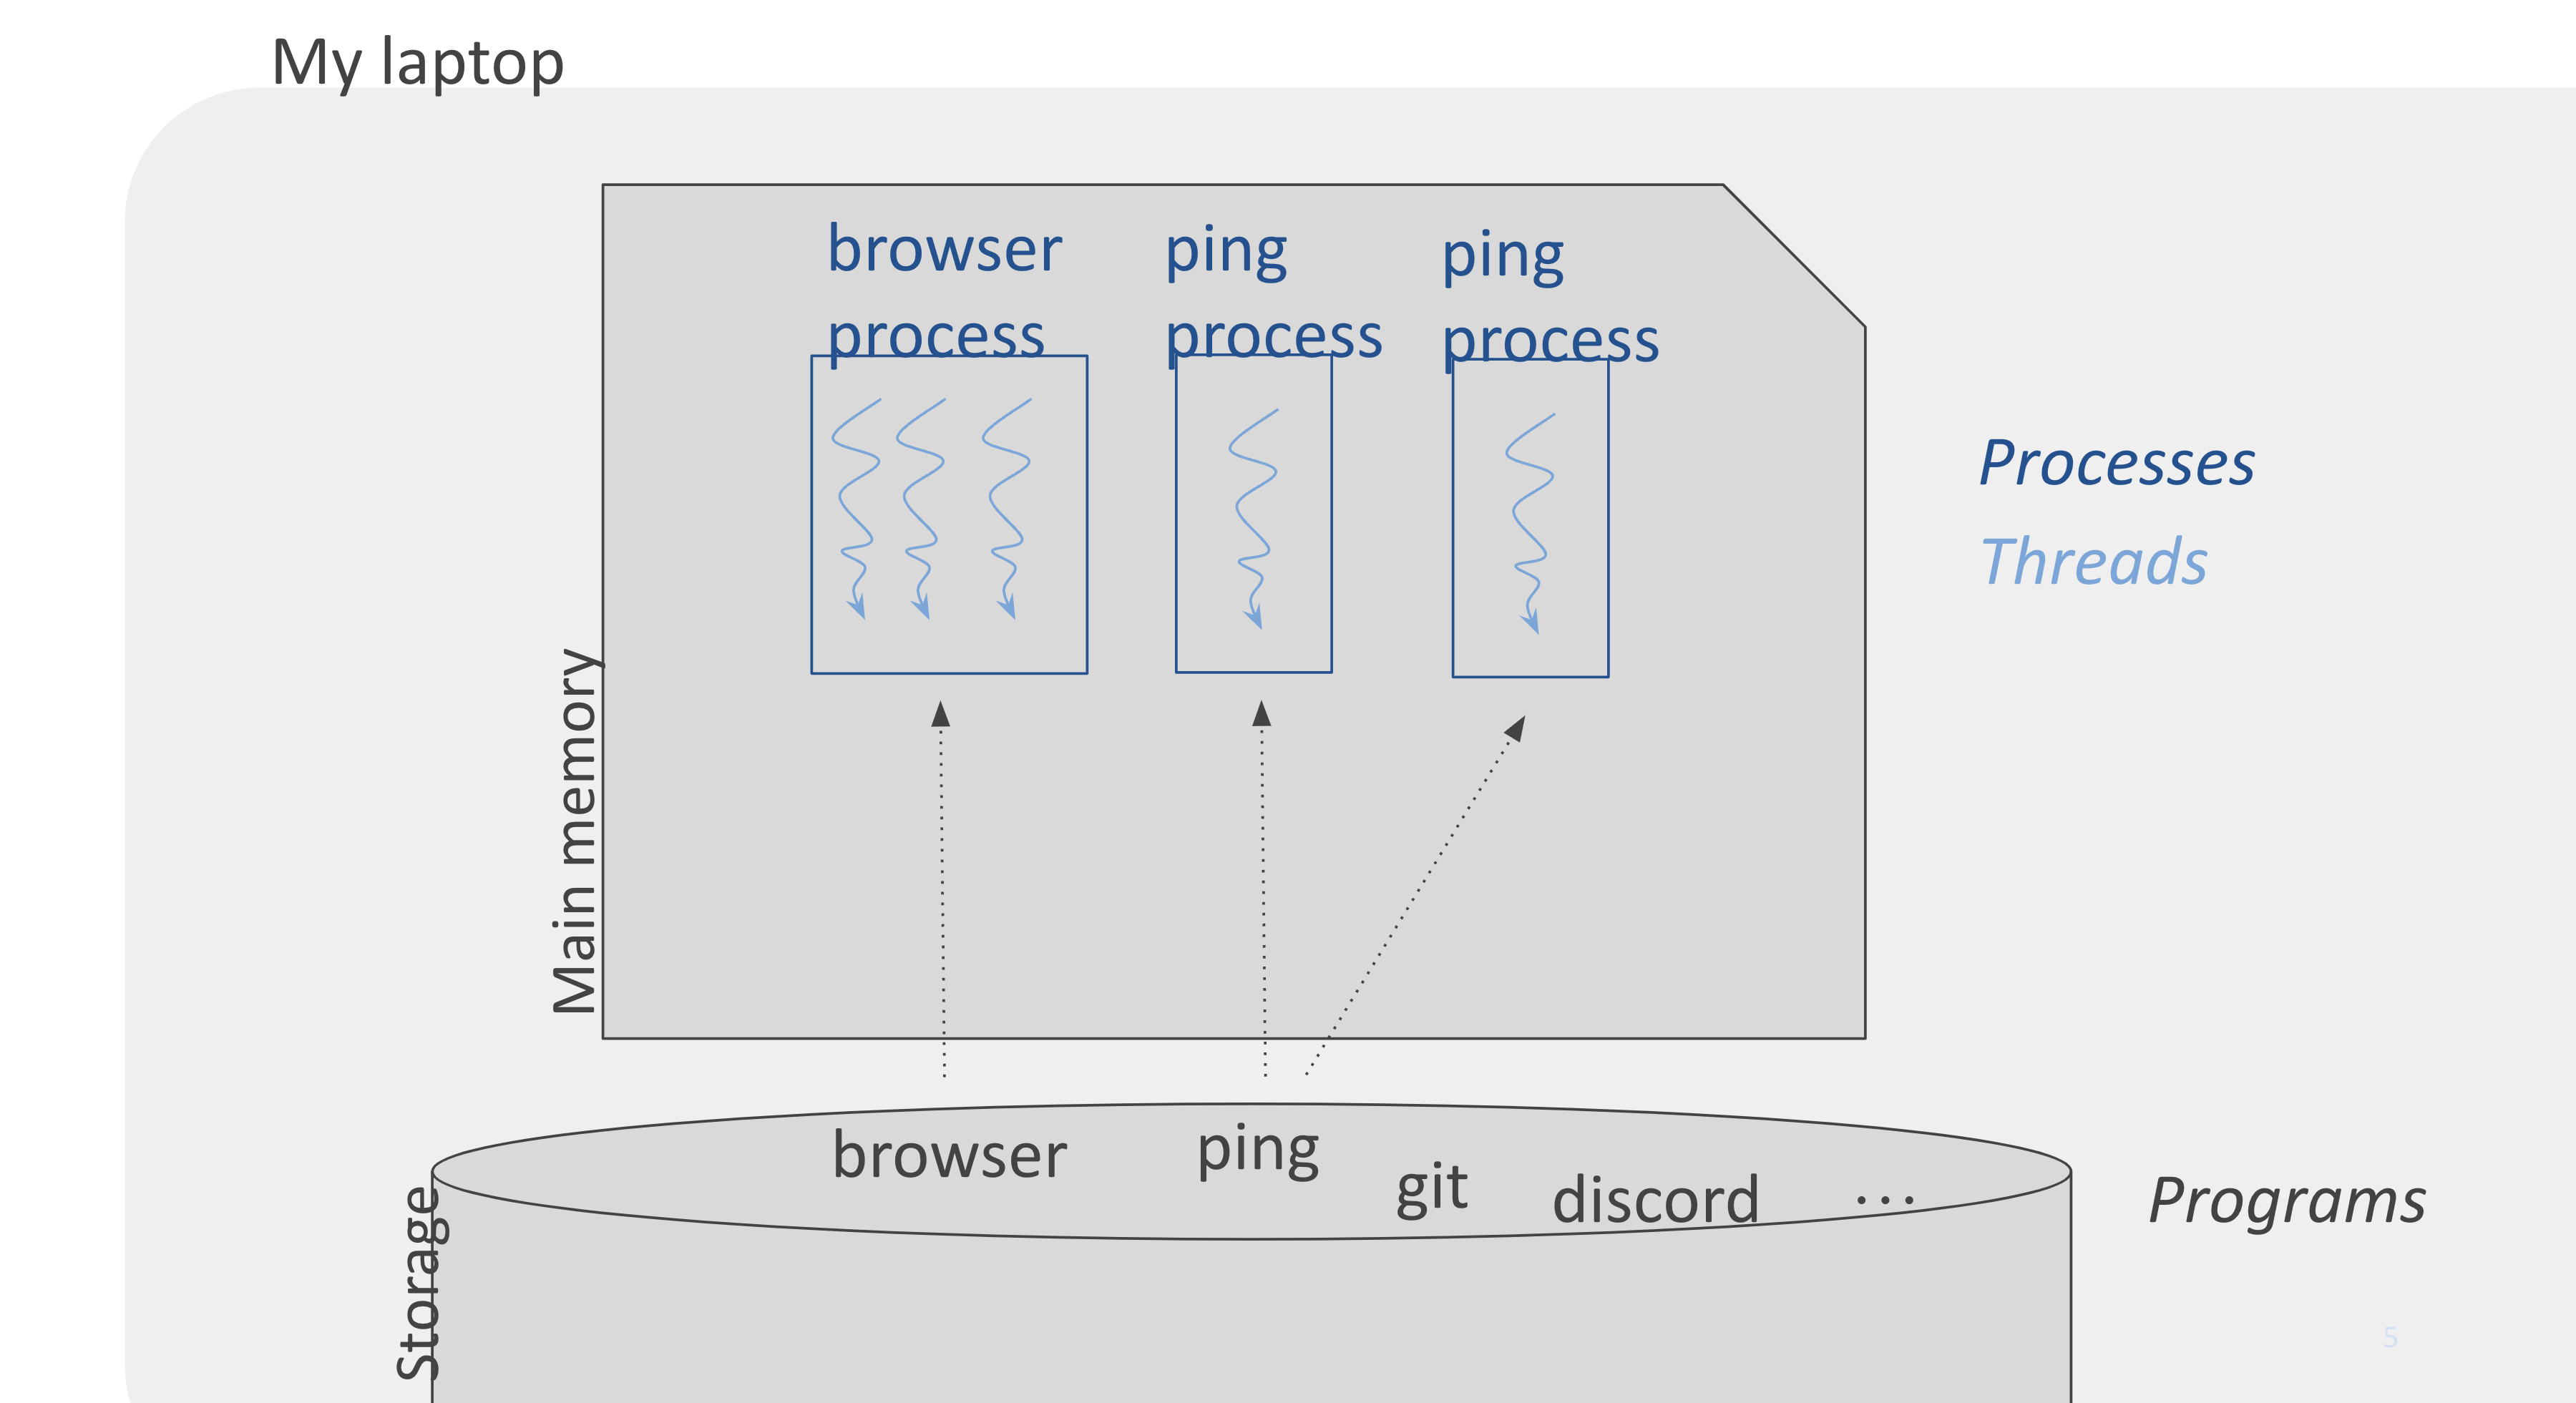
\includegraphics[width=1.2\textwidth]{chapters/L1/images/threads.png}
\end{center}
\end{minipage}\vfill
\vfill
\begin{definition}[Program, Process, Thread]
A \textbf{program} is a set of instructions stored as a file on disk. When a program is invoked, the computer creates a \textbf{process}—a running instance of that program in main memory. A process may consist of one or more \textbf{threads}, which are the individual sequences of execution within the process.
\end{definition}

%%%%%%%%%%%%%%%%%%%%%%%%%%%%%%%%%%%%%%%%%%%%%%%%%%%%%%%%%%%%%%%%%%%%%jjjj%
\vfill
\subsection{Accessing a Video: A Distributed Application}

When you use your web browser to access a video, the browser sends a message (or request) to a remote YouTube server. The browser process (running on your laptop) and the server process (running on a different computer) work together as parts of a \emph{distributed application}. 
\begin{center}
  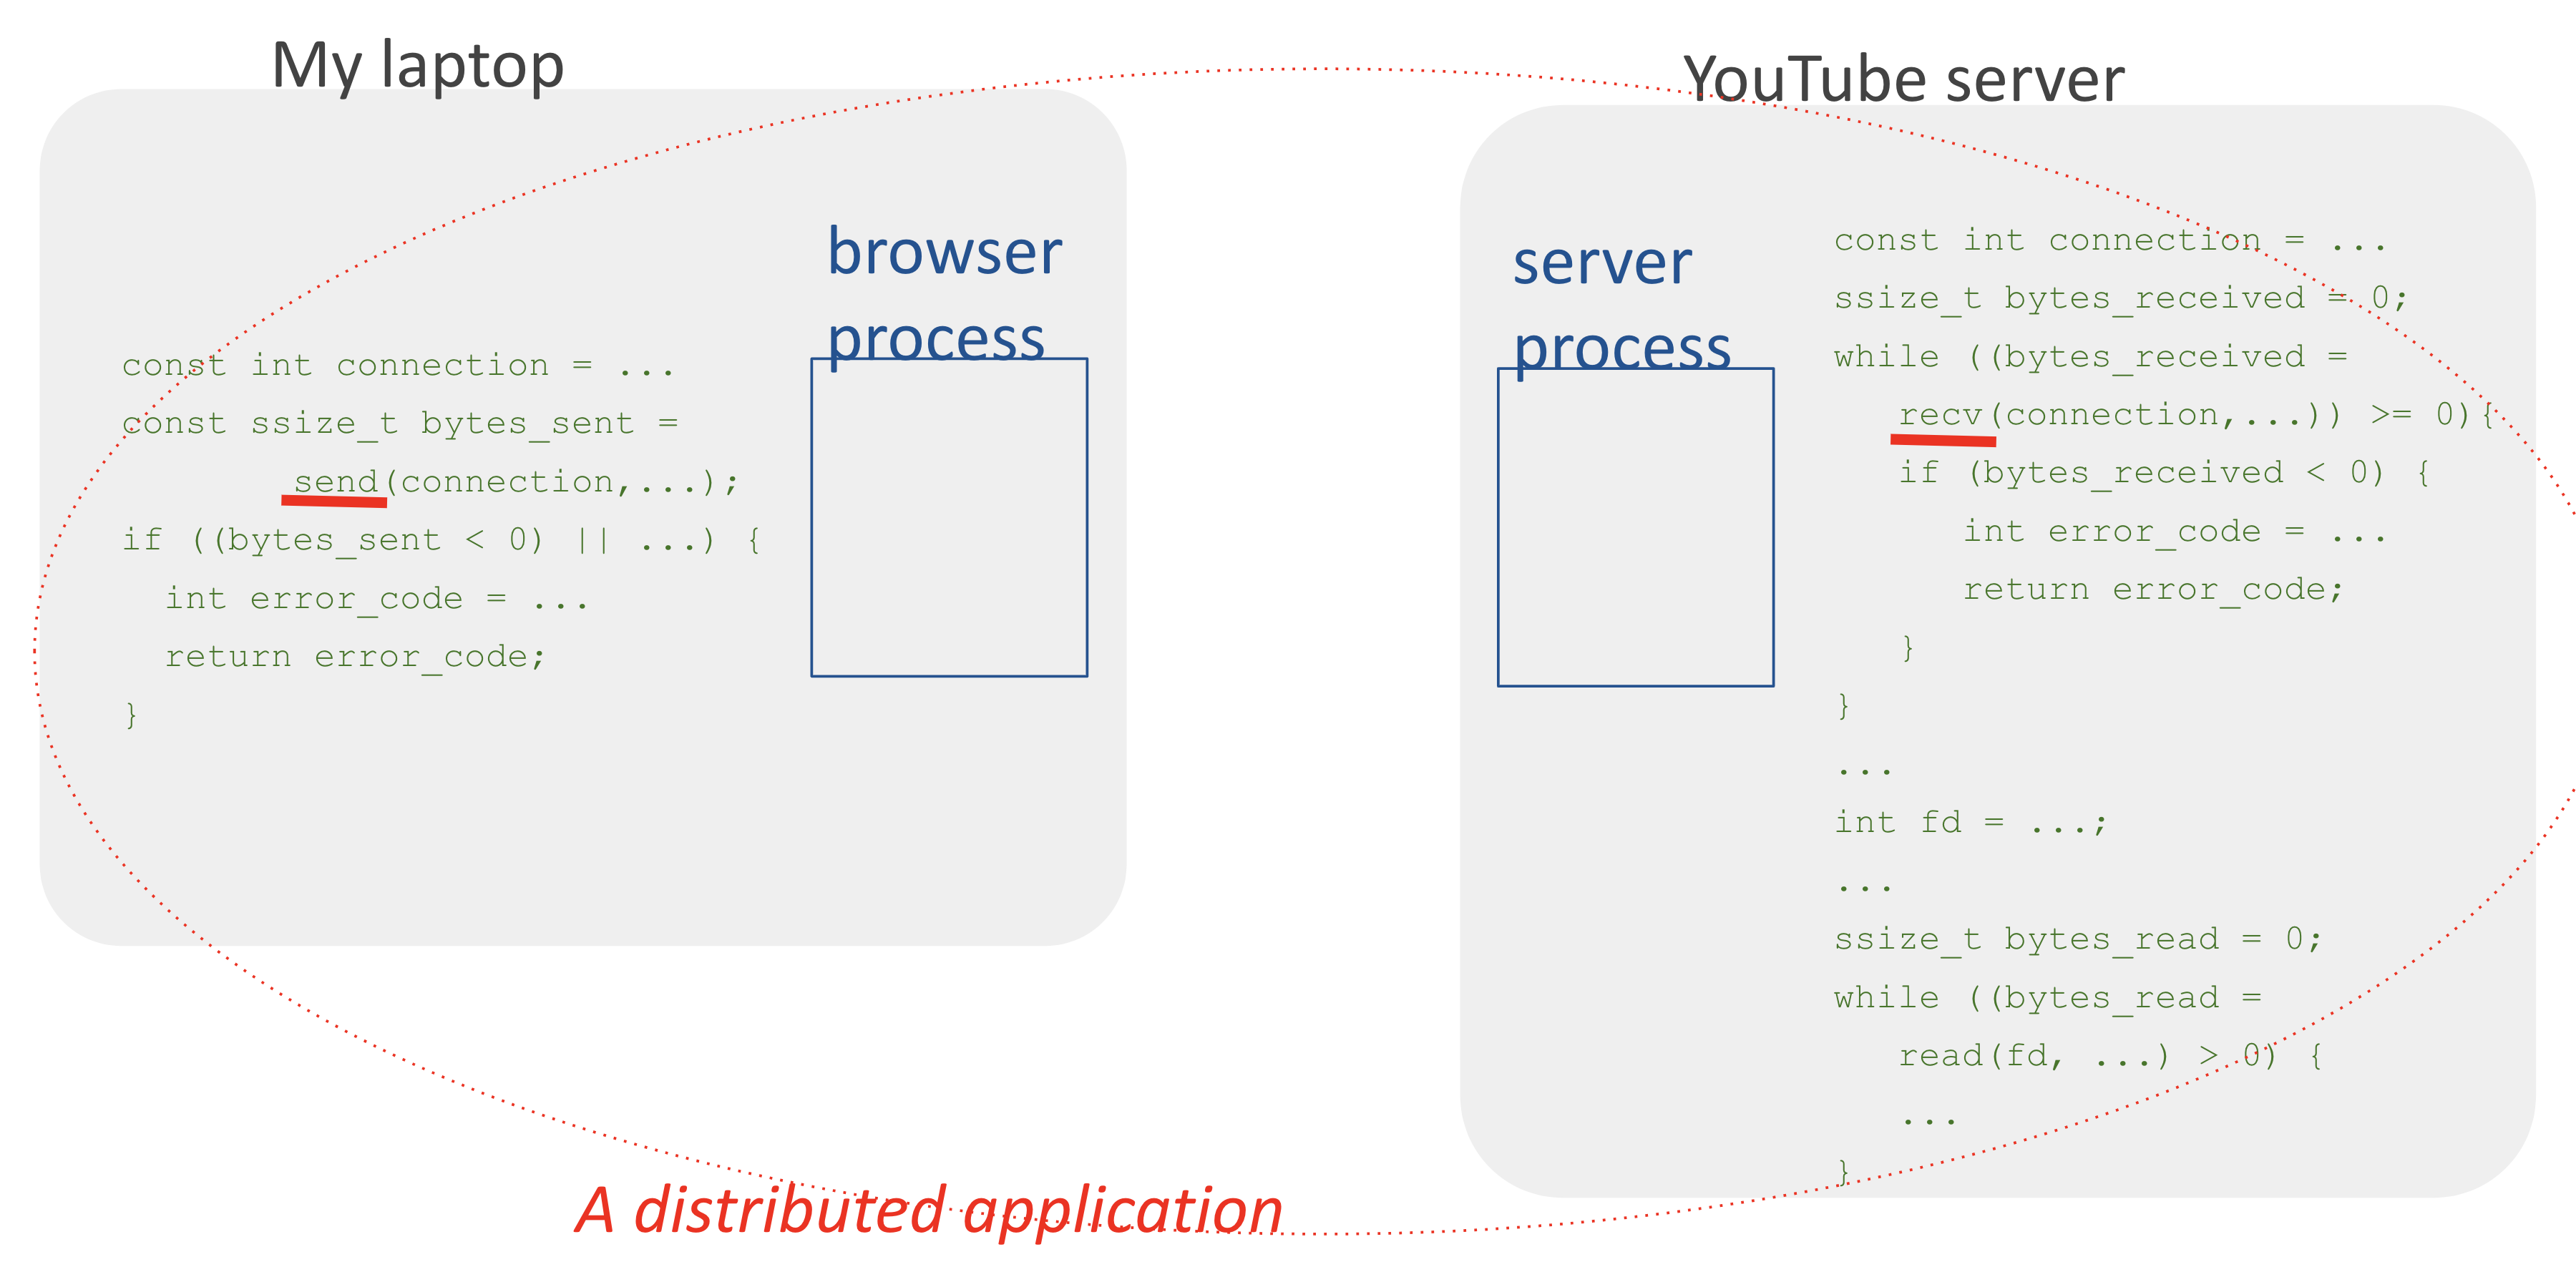
\includegraphics[width=0.95\textwidth]{chapters/L1/images/distributed.png}
\end{center}

%%%%%%%%%%%%%%%%%%%%%%%%%%%%%%%%%%%%%%%%%%%%%%%%%%%%%%%%%%%%%%%%%%%%%%
\newpage
\subsection{Communication Protocols}
For two processes running on different devices to work together, they must follow a predetermined set of rules known as a \textbf{communication protocol}. For example, a simple protocol might involve:
\begin{itemize}
  \item[-] One process sending “hello” and waiting for a “hello back.”
  \item[-] A subsequent request for a specific file (e.g., \texttt{xyz}) with the server responding with the file or an error message.
\end{itemize}
Much like human communication, these protocols ensure that both parties know what to expect, enabling effective interaction.

\begin{center}
  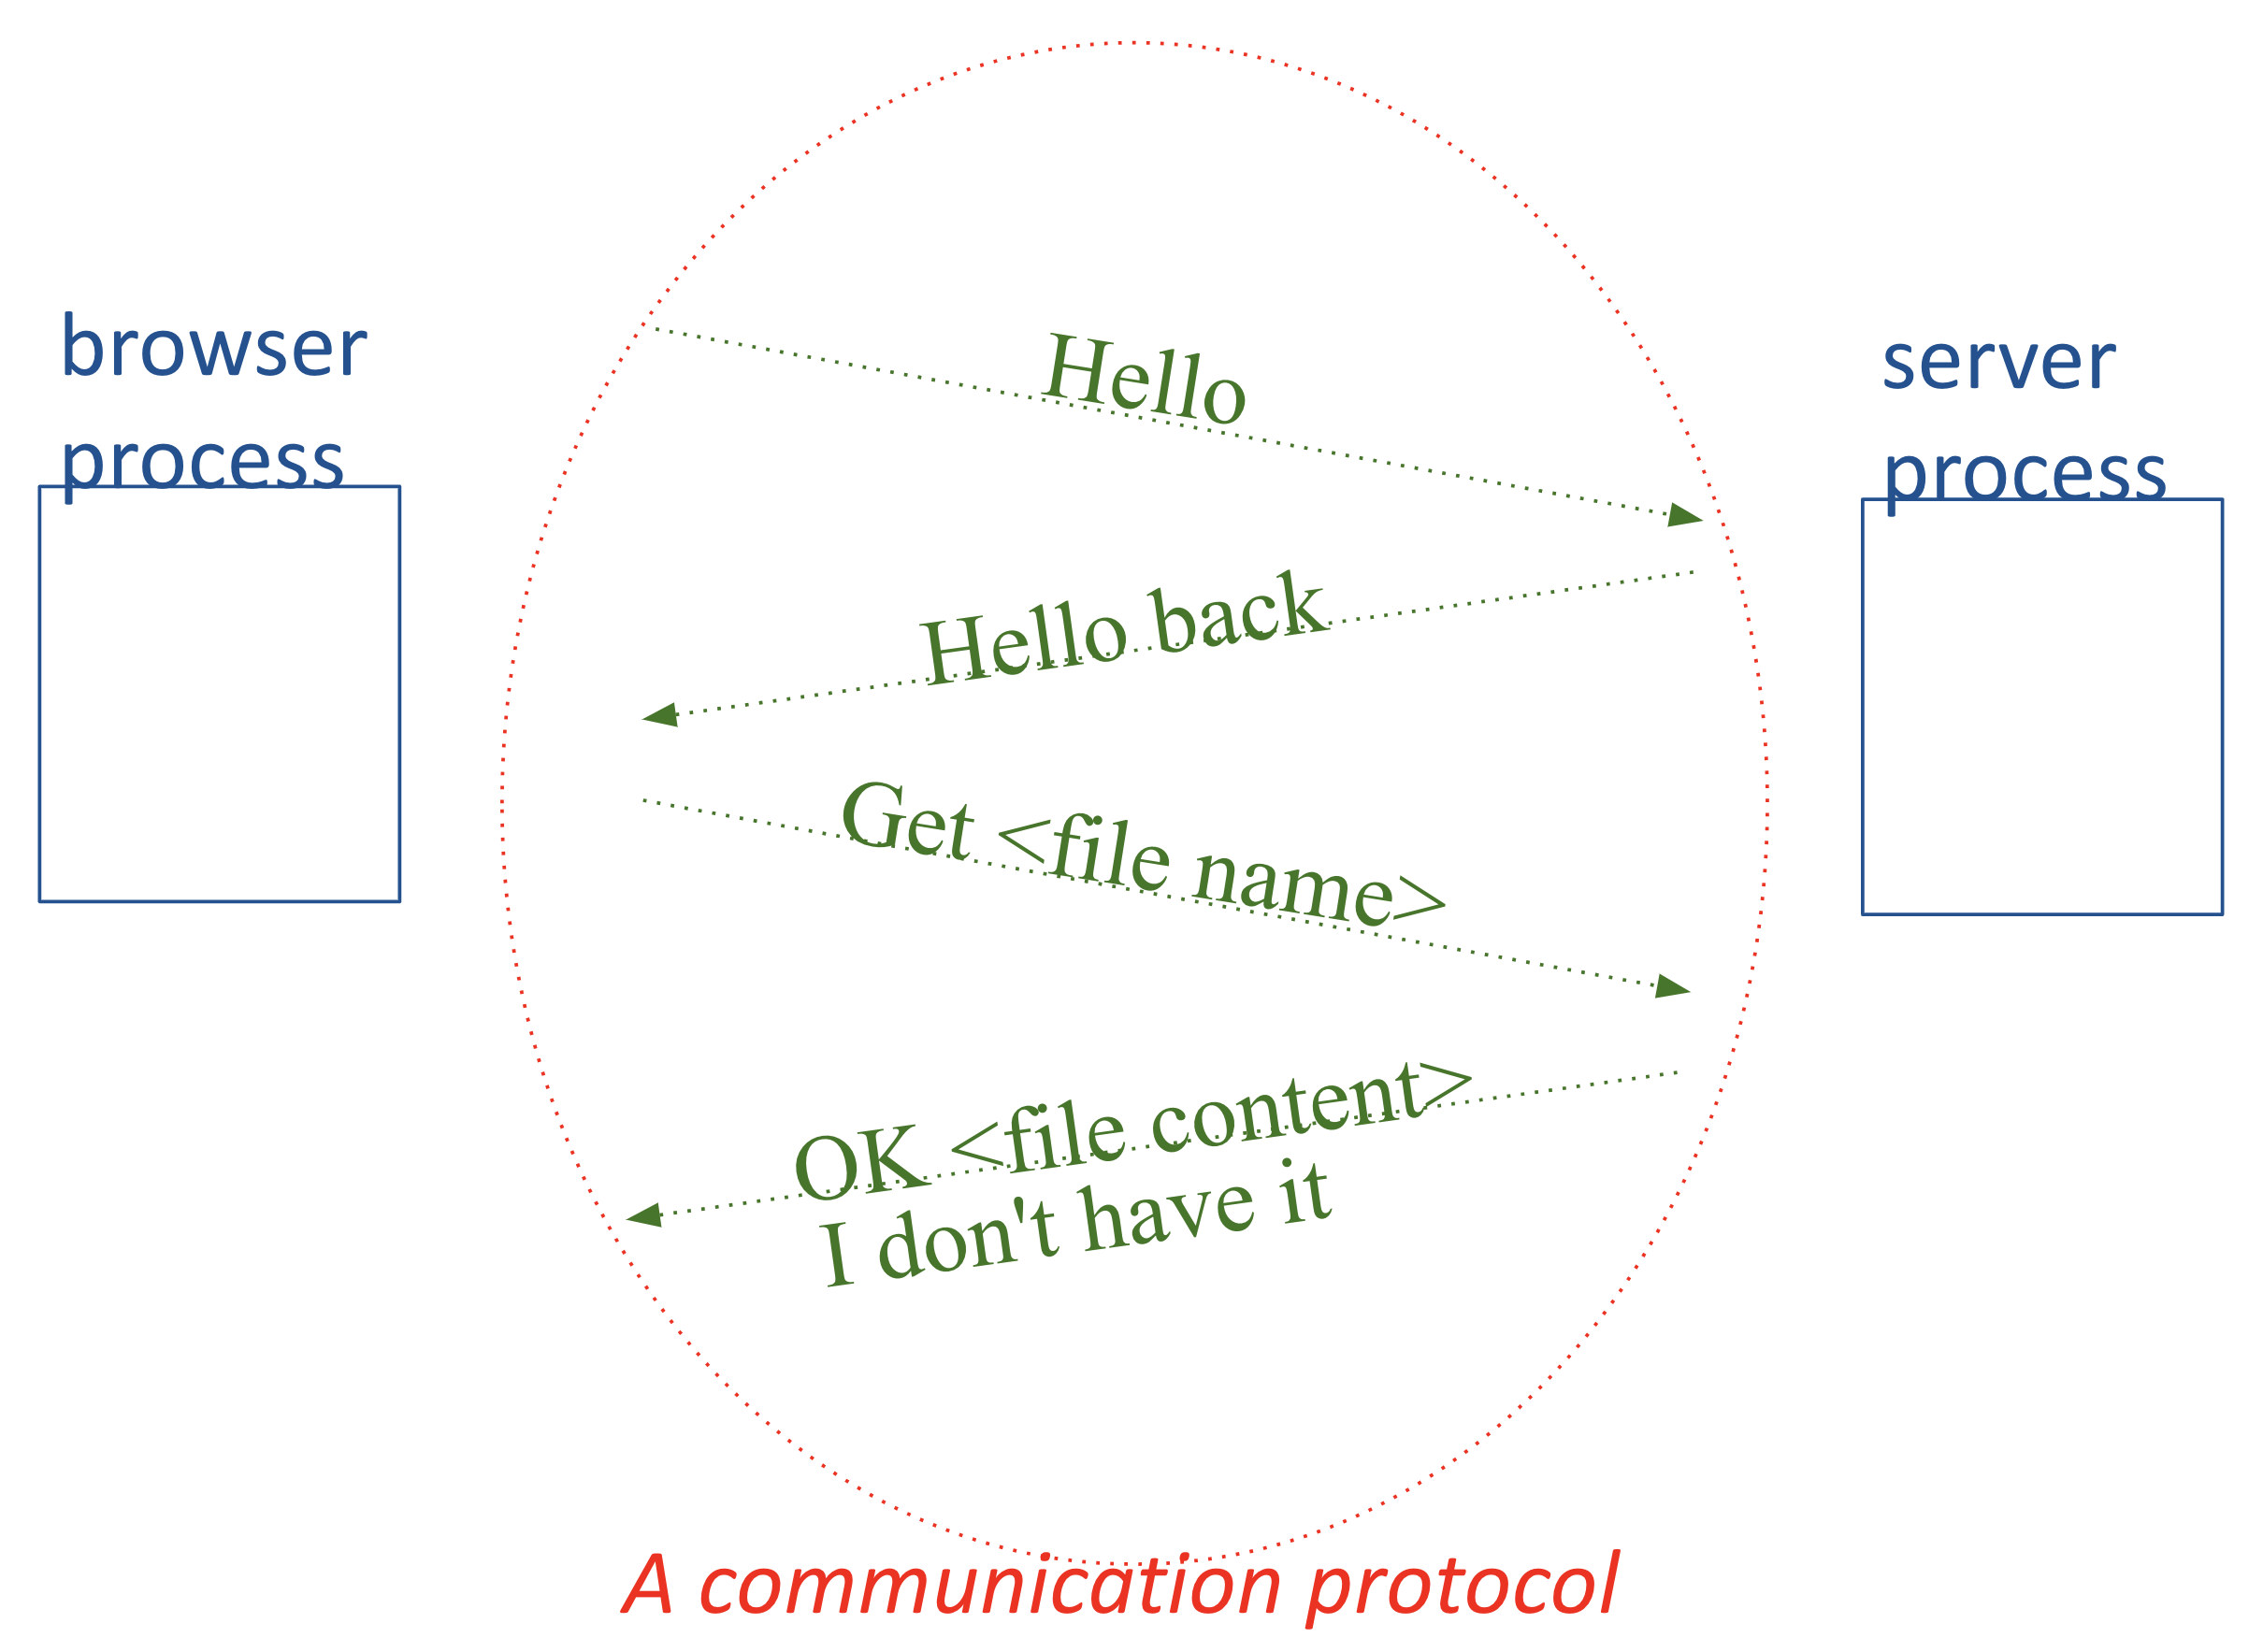
\includegraphics[width=0.45\textwidth]{chapters/L1/images/comm_prot.png}
\end{center}

%%%%%%%%%%%%%%%%%%%%%%%%%%%%%%%%%%%%%%%%%%%%%%%%%%%%%%%%%%%%%%%%%%%%%%
\subsection{Distributed Applications and APIs}

Distributed applications consist of separate pieces of code running as processes on different machines but working toward a common goal. These processes exchange messages over the Internet by following communication protocols.  
To simplify the development of these applications, developers use \emph{system calls} (or \textbf{syscalls}). Syscalls are special functions provided by the operating system that allow processes to access resources (e.g., network and storage) without needing to know the low-level details.

The set of syscalls available to an application forms its \textbf{Application Programming Interface} (API), abstracting away the complexities of resource management.

\begin{center}
  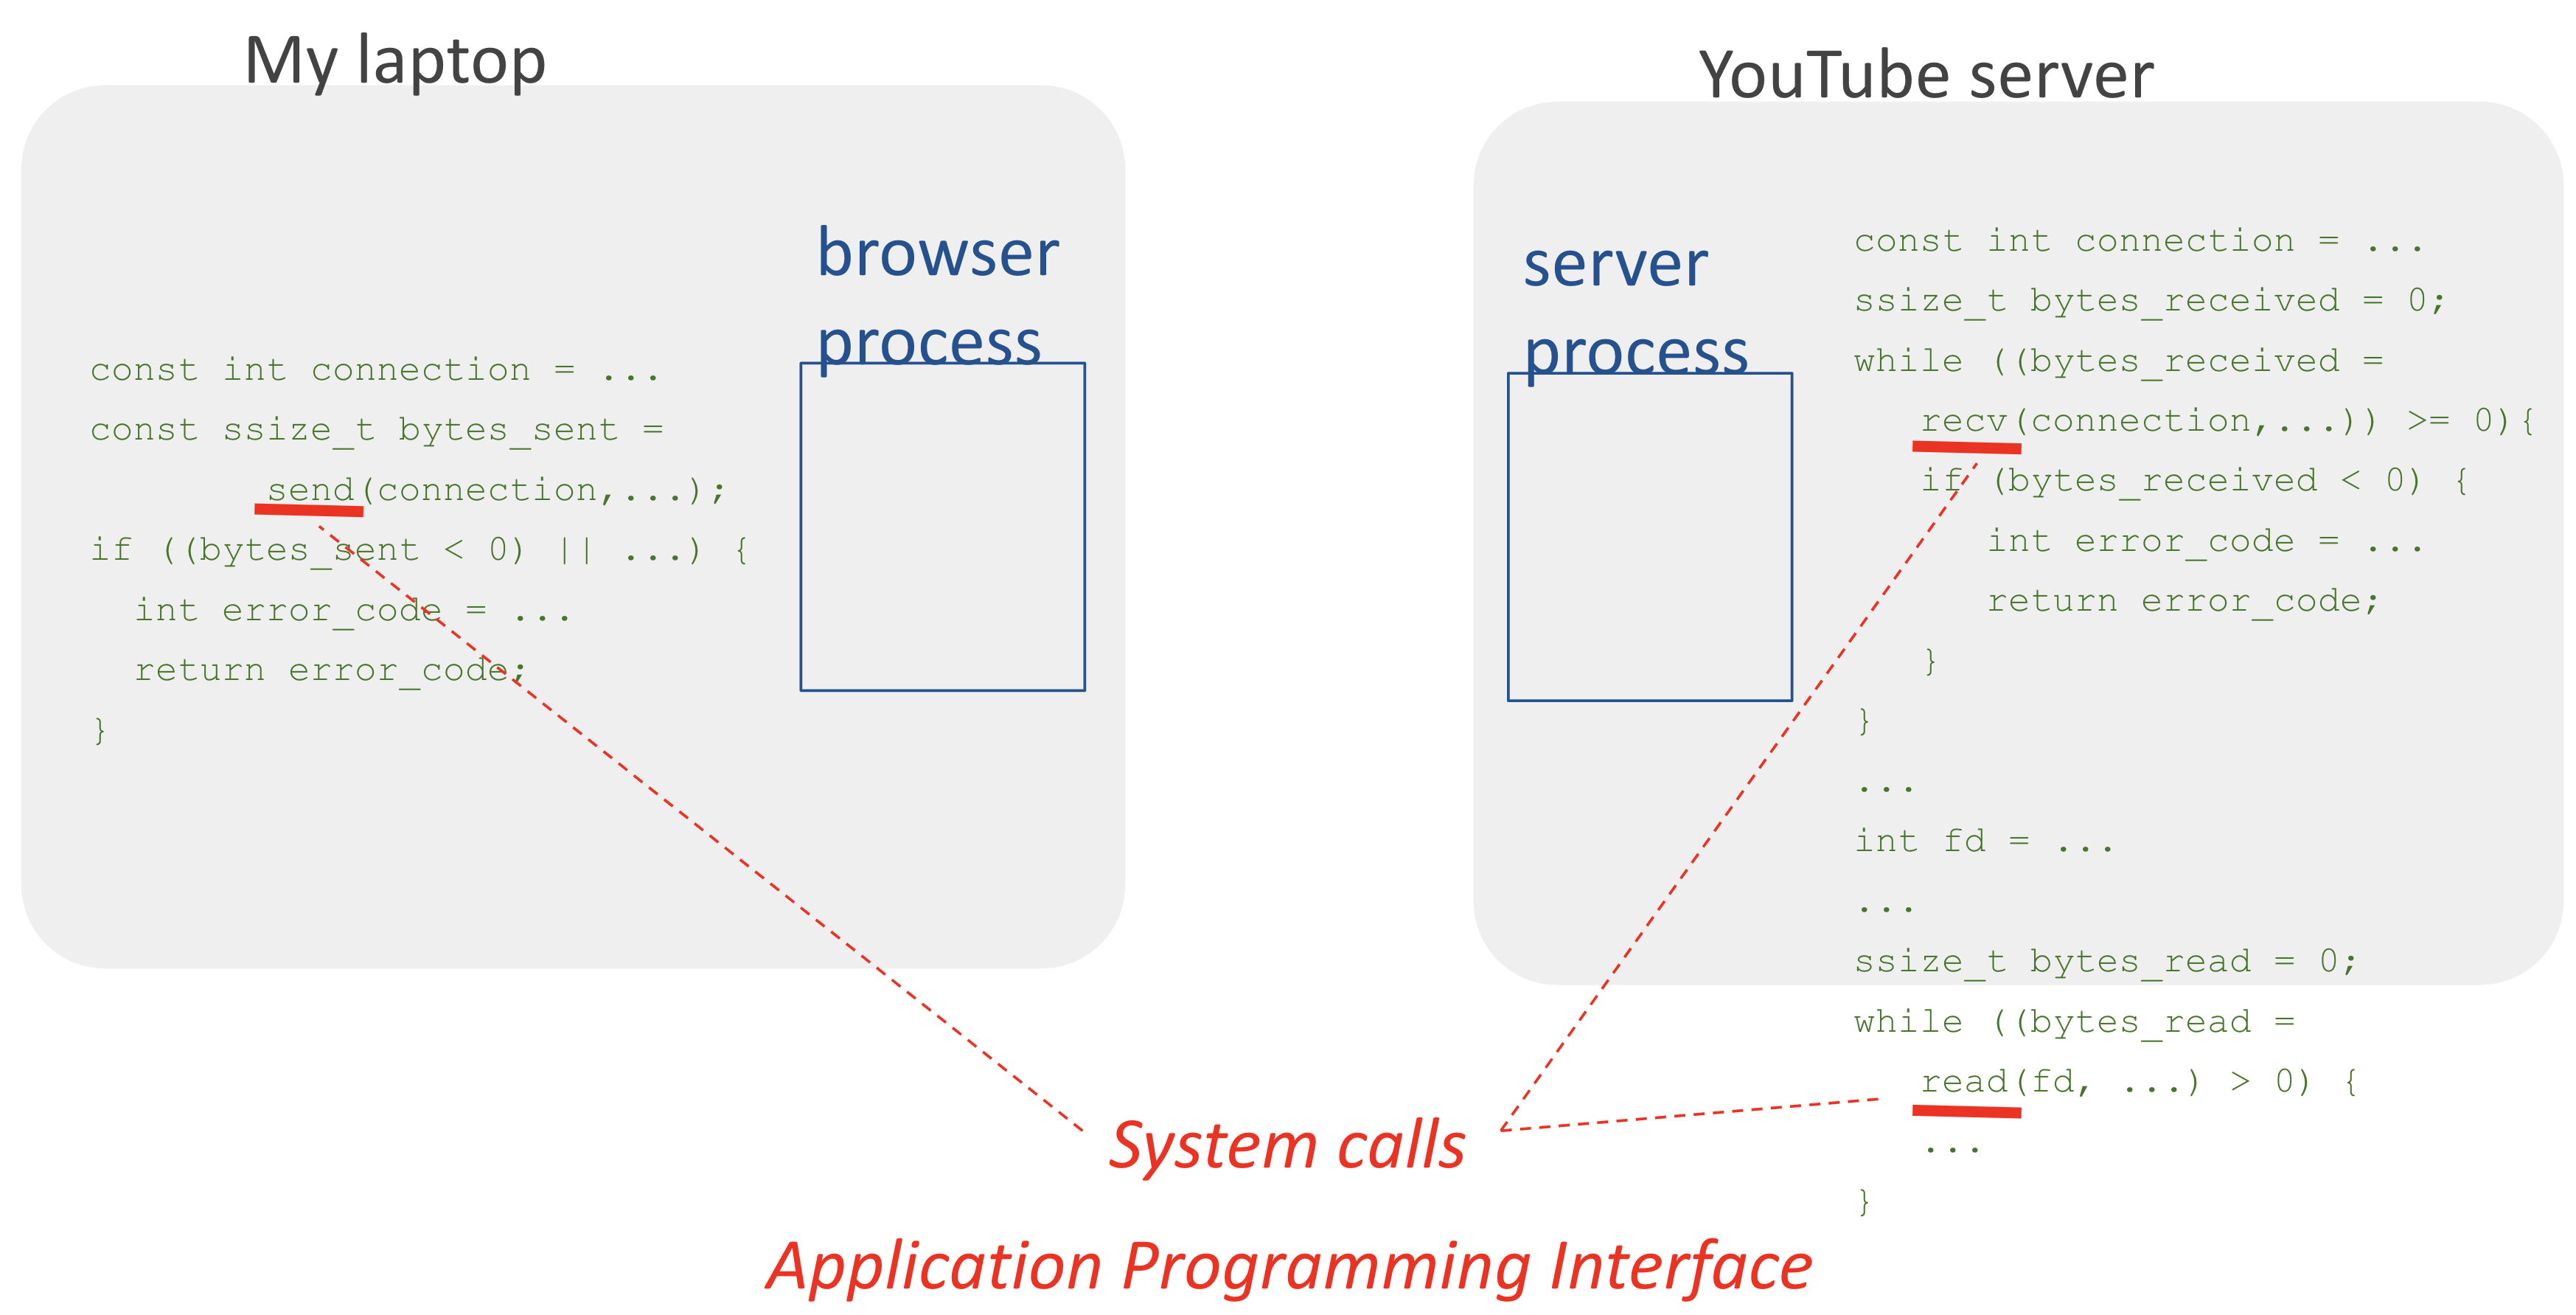
\includegraphics[width=0.85\textwidth]{chapters/L1/images/api.png}
\end{center}

%%%%%%%%%%%%%%%%%%%%%%%%%%%%%%%%%%%%%%%%%%%%%%%%%%%%%%%%%%%%%%%%%%%%%%
\vfill
\begin{definition}[Interface]
An \textbf{interface} is a set of rules that defines how different components communicate. For instance, when sending a letter via the postal system, one must follow specific rules (e.g., write the address and affix a stamp). This interface abstracts the complexities of the postal system so that users do not need to understand its internal operations.
\end{definition}

\begin{center}
  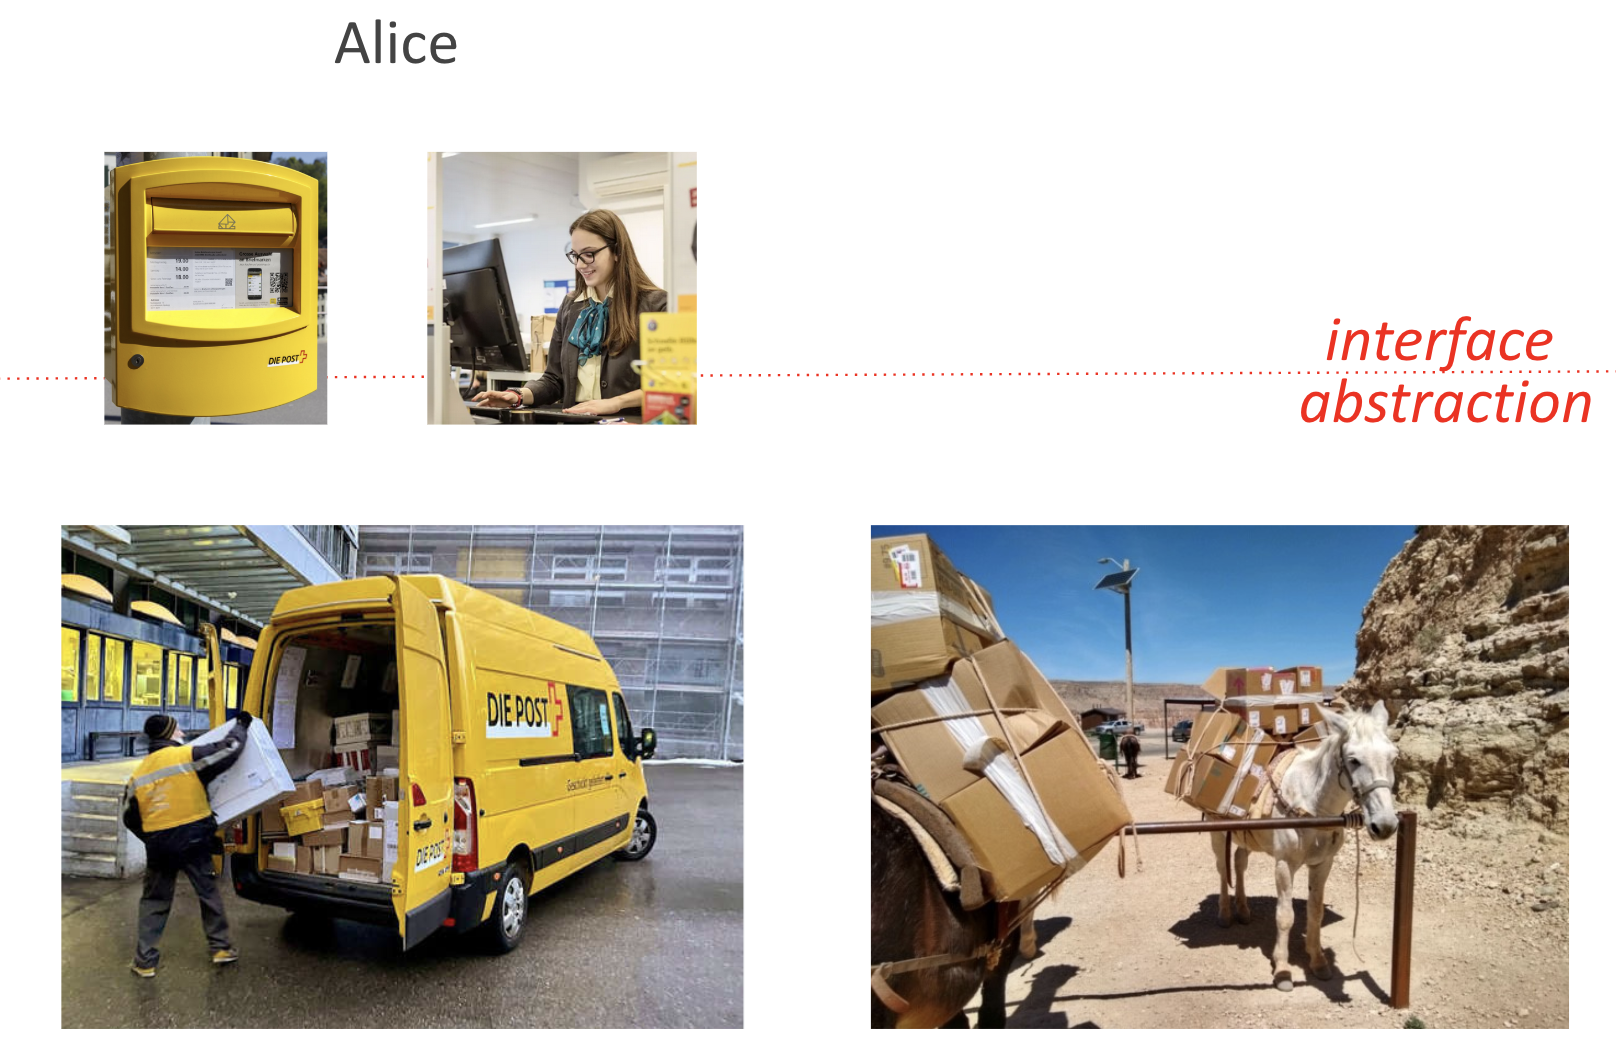
\includegraphics[width=0.65\textwidth]{chapters/L1/images/postal.png}
\end{center}
\vfill
%%%%%%%%%%%%%%%%%%%%%%%%%%%%%%%%%%%%%%%%%%%%%%%%%%%%%%%%%%%%%%%%%%%%%%
\subsection{System Calls (Syscalls)}

Syscalls form the interface between a process and external resources (like network and storage). They provide an abstraction of these resources, allowing a process to use them without knowing their intricate details. For example, when a process makes a syscall such as \texttt{send} or \texttt{recv}, the operating system’s network stack handles the details of the communication.

\begin{center}
  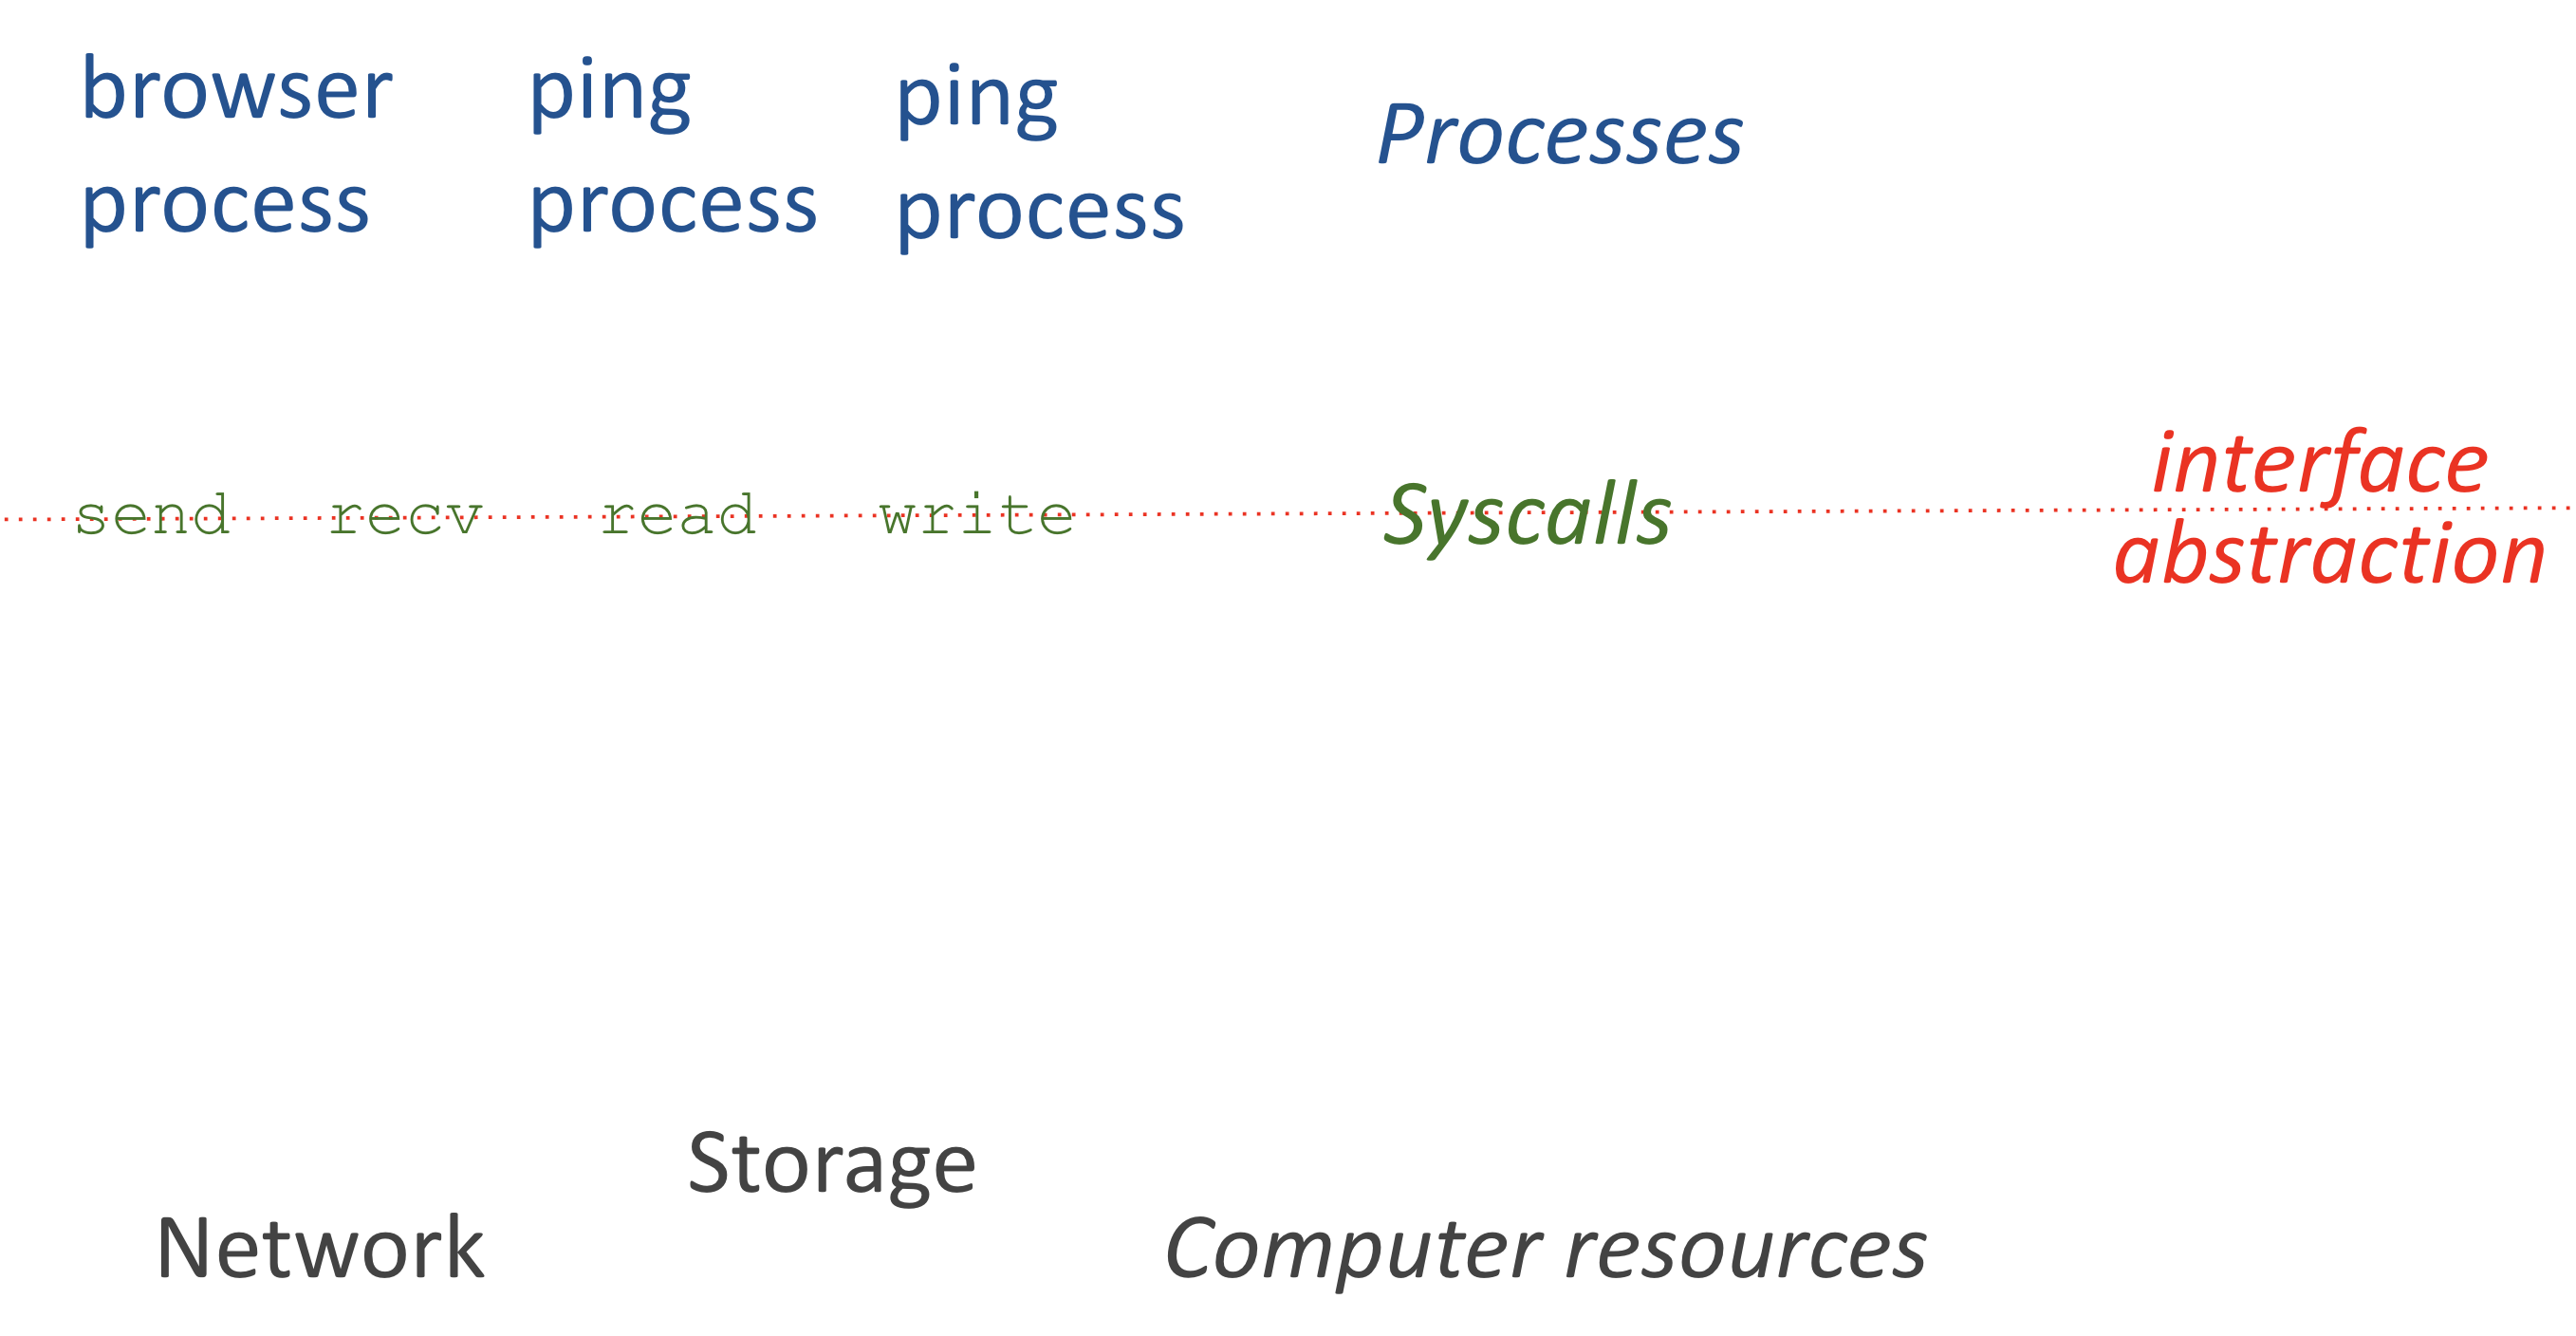
\includegraphics[width=0.65\textwidth]{chapters/L1/images/syscalls.png}
\end{center}
\vfill
\newpage
%%%%%%%%%%%%%%%%%%%%%%%%%%%%%%%%%%%%%%%%%%%%%%%%%%%%%%%%%%%%%%%%%%%%%%
\section{The Operating System}
Conceptually, the OS sits between running processes and the underlying hardware resources. It provides the syscall interface and handles tasks such as file system management and network communication. \\
\begin{minipage}{0.45\textwidth}
\begin{center}
  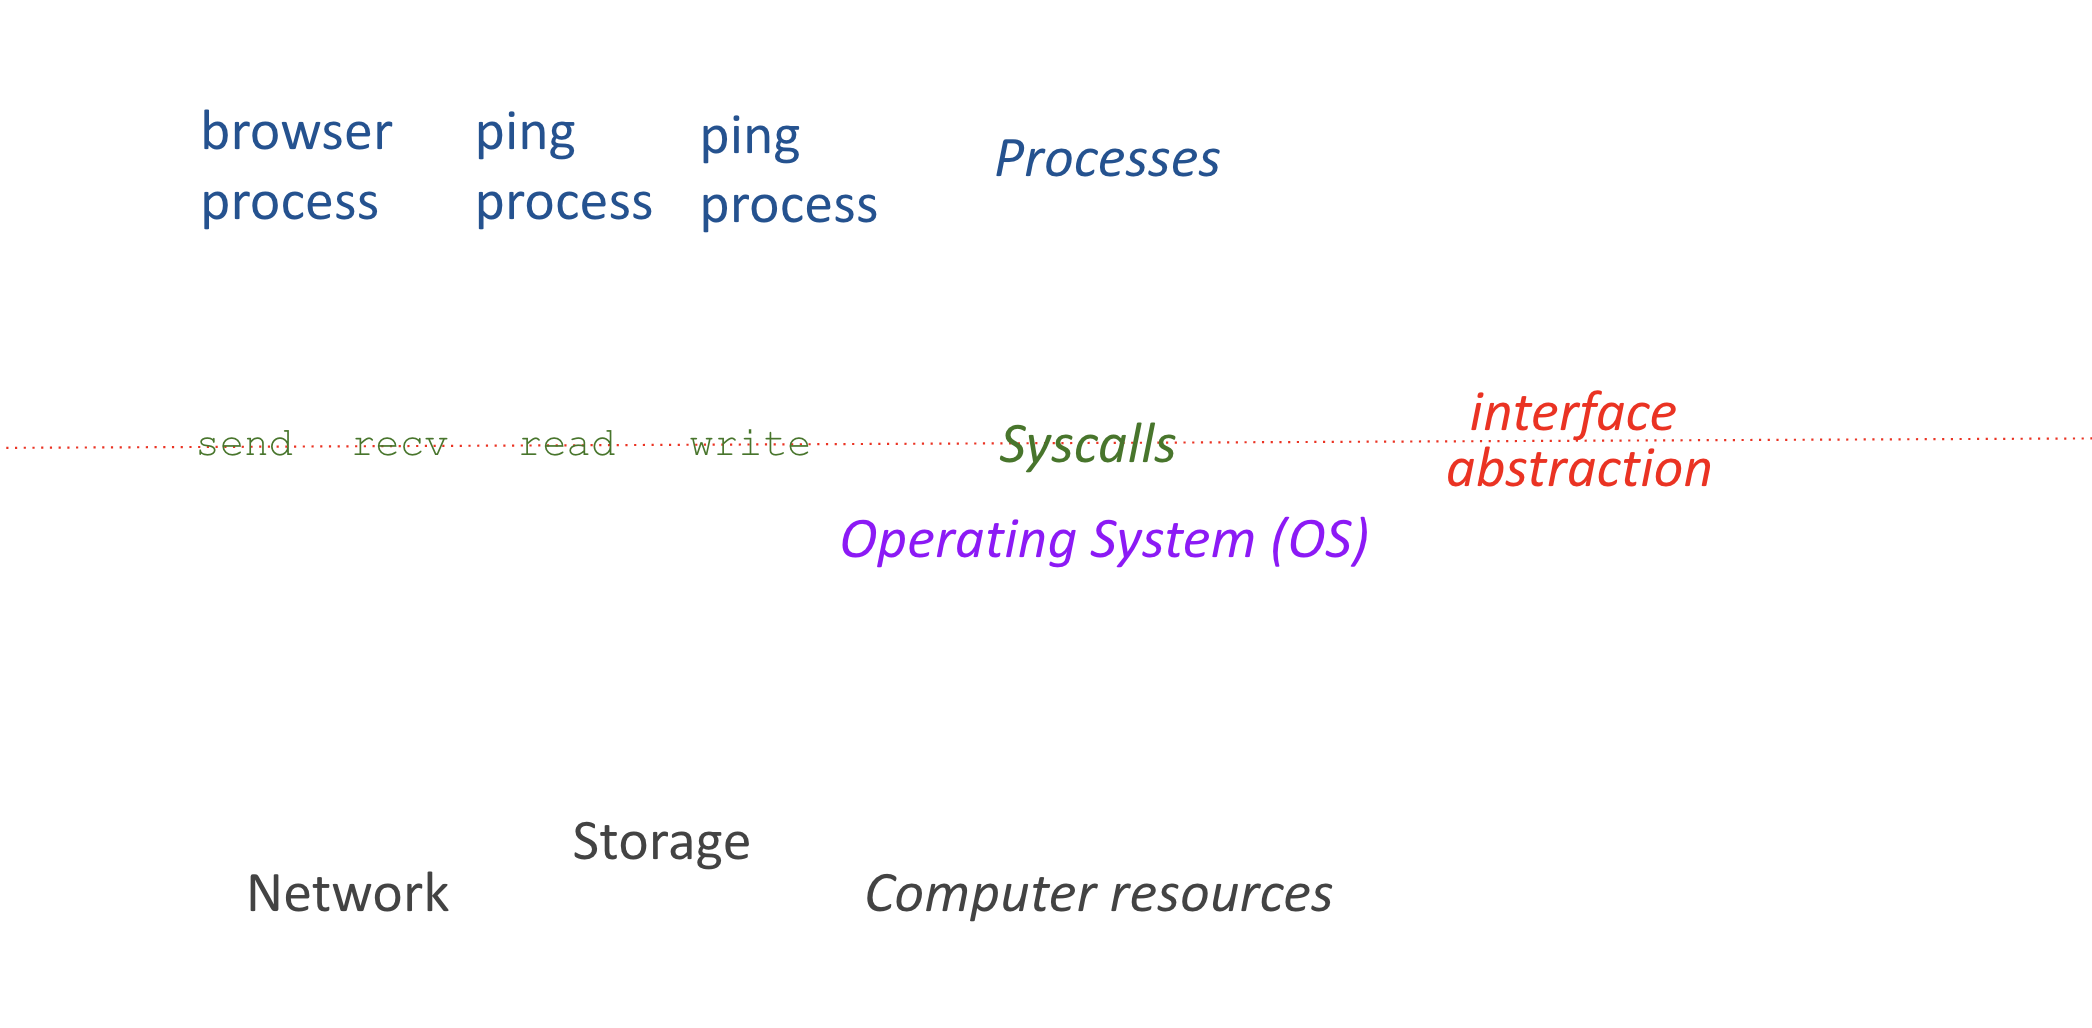
\includegraphics[width=1.15\textwidth]{chapters/L1/images/isa_os.png}
\end{center}
\end{minipage}
\hfill
\vline
\hfill
\begin{minipage}{0.45\textwidth}
\begin{center}
  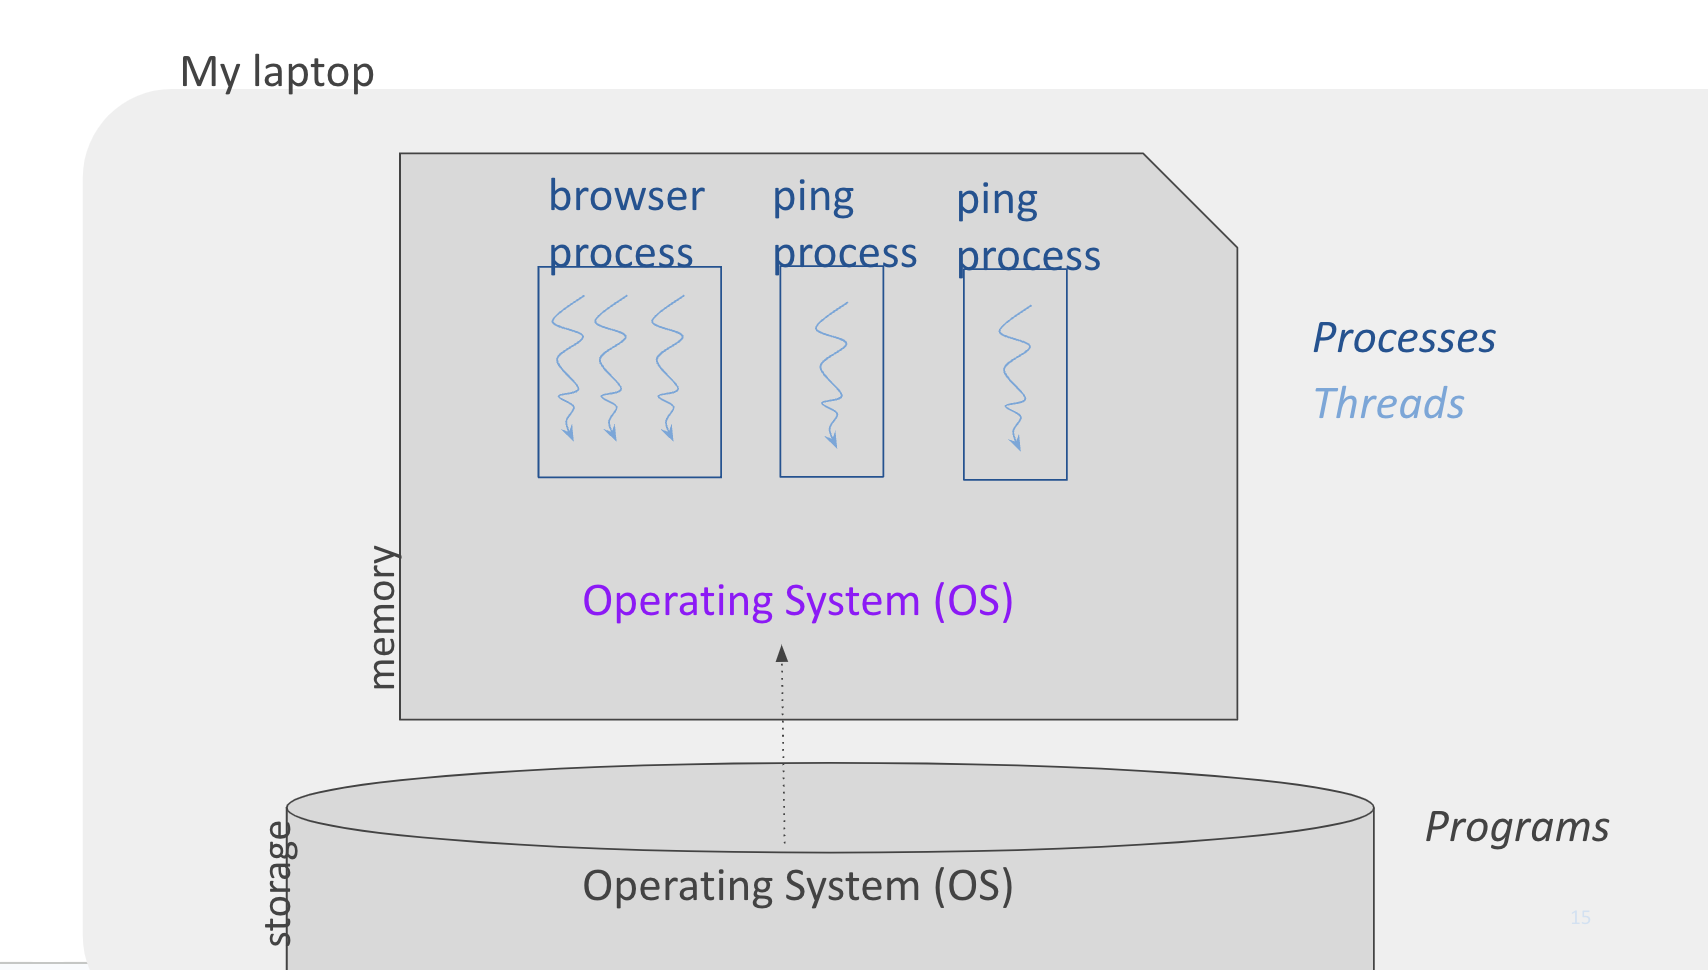
\includegraphics[width=1.15\textwidth]{chapters/L1/images/os.png}
\end{center}
\end{minipage}

\subsection{Example: Execution When Fetching a Video from YouTube}
When you click a YouTube link, the following sequence of events occurs:
\begin{enumerate}
  \item Your trackpad detects the click and notifies the OS.
  \item The OS identifies that the click occurred within the web browser window and alerts the corresponding process.
  \item The browser process initiates a chain of events that eventually fetches and displays the video.
\end{enumerate}

\begin{center}
  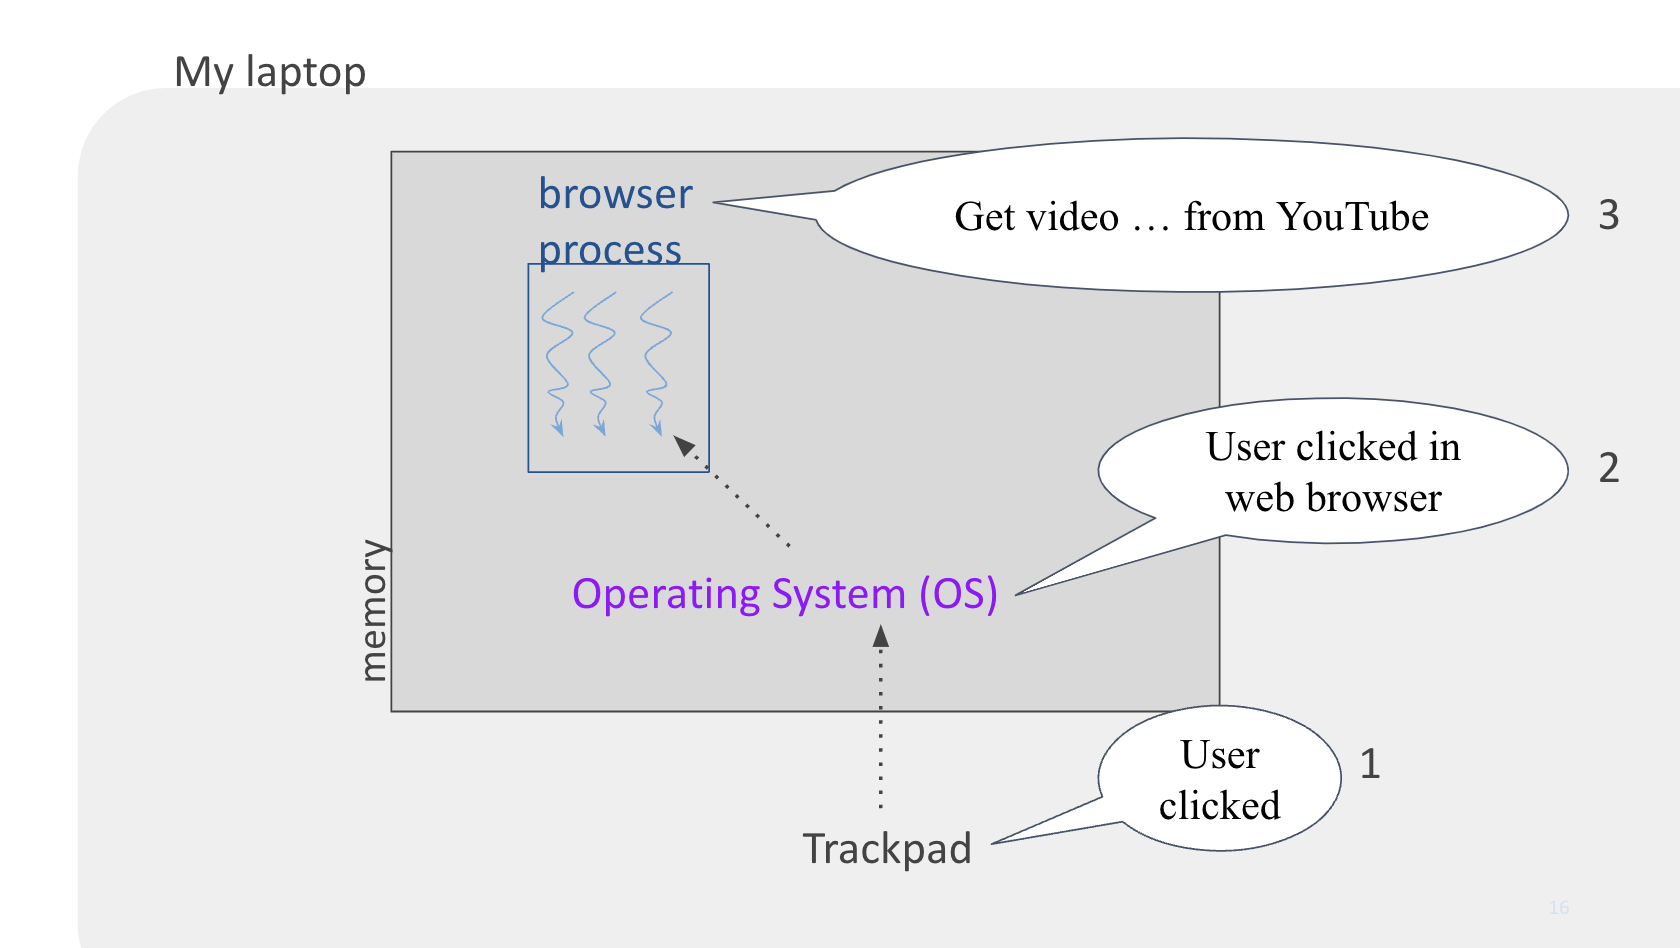
\includegraphics[width=0.85\textwidth]{chapters/L1/images/os_youtube.png}
\end{center}

\newpage
%%%%%%%%%%%%%%%%%%%%%%%%%%%%%%%%%%%%%%%%%%%%%%%%%%%%%%%%%%%%%%%%%%%%%%
\section{Program and ISA}
\subsection{Program}
A \textbf{program} is a set of instructions written by a human in a high-level programming language (such as C, Java, or Python) that implements an algorithm. When compiled, a program is translated into an \emph{executable} (or binary) that the CPU can run. The executable is expressed in the language defined by the computer's \textbf{Instruction Set Architecture} (ISA).

\begin{center}
  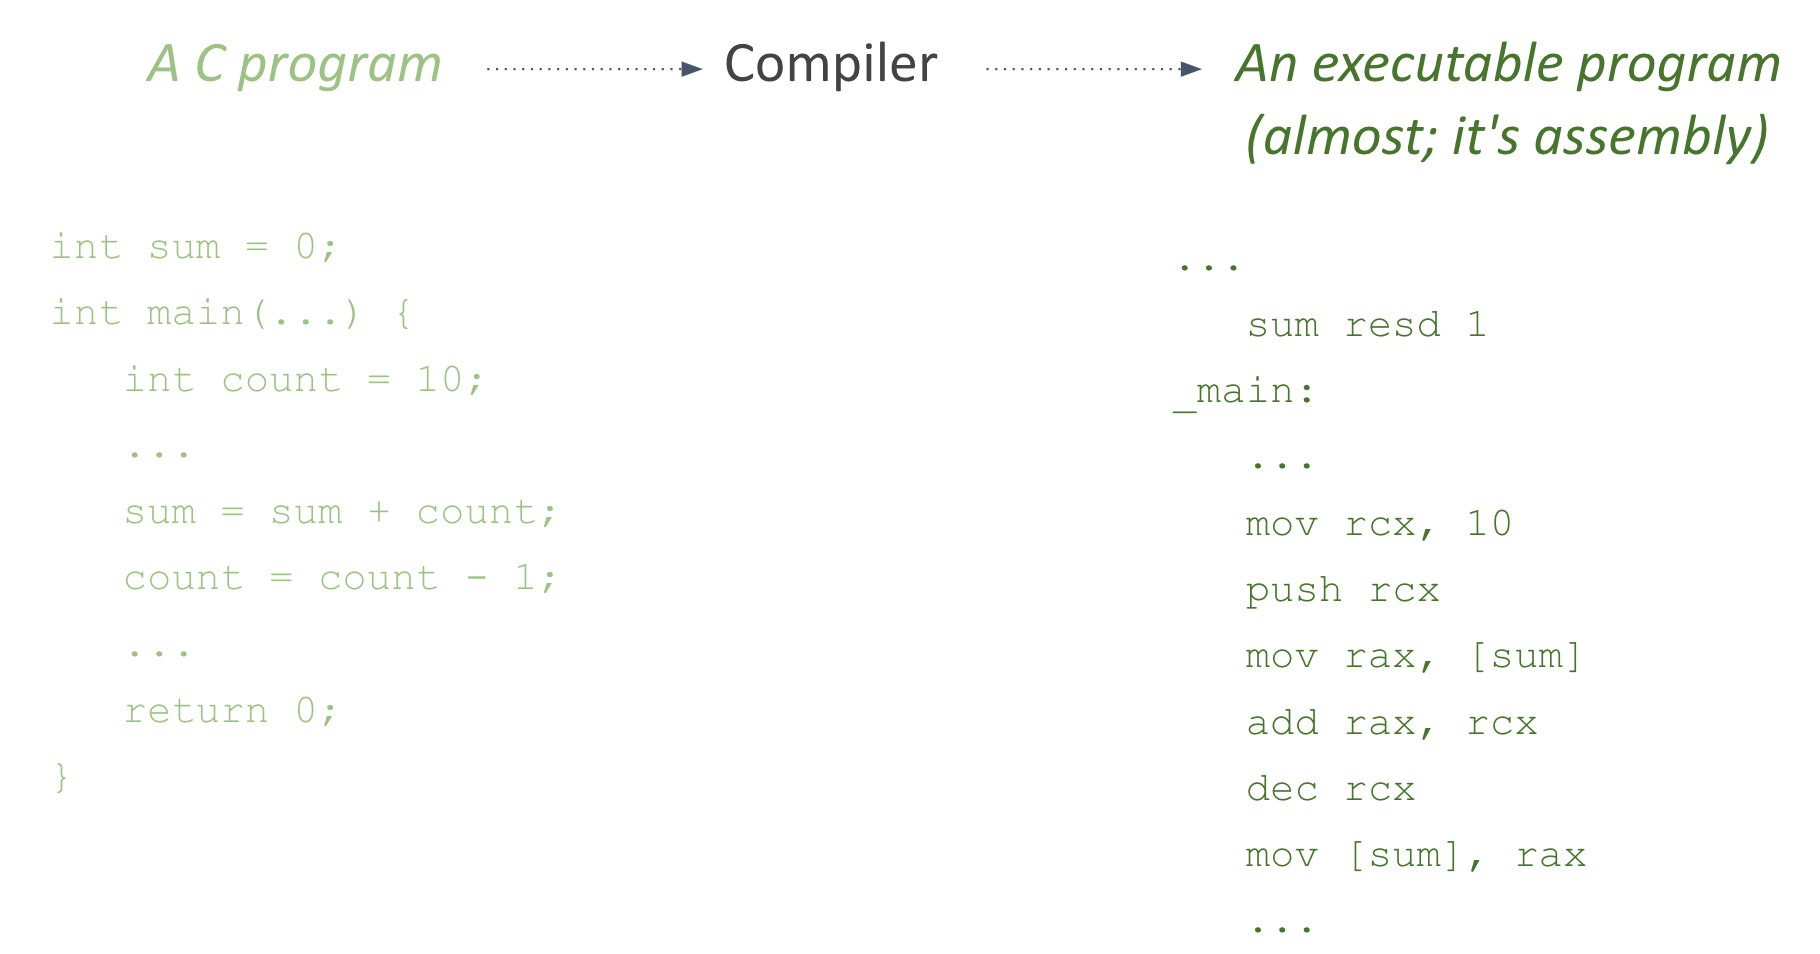
\includegraphics[width=0.75\textwidth]{chapters/L1/images/program.png}
\end{center}

\begin{minipage}{0.45\textwidth}
\begin{definition}[ISA]
The \textbf{Instruction Set Architecture} (ISA) is the set of all instructions that a CPU can understand and execute. It forms an interface between the compiler (which translates high-level code into machine code) and the CPU.
\end{definition}
\end{minipage}
\hfill
\vline
\hfill
\begin{minipage}{0.45\textwidth}
\begin{center}
  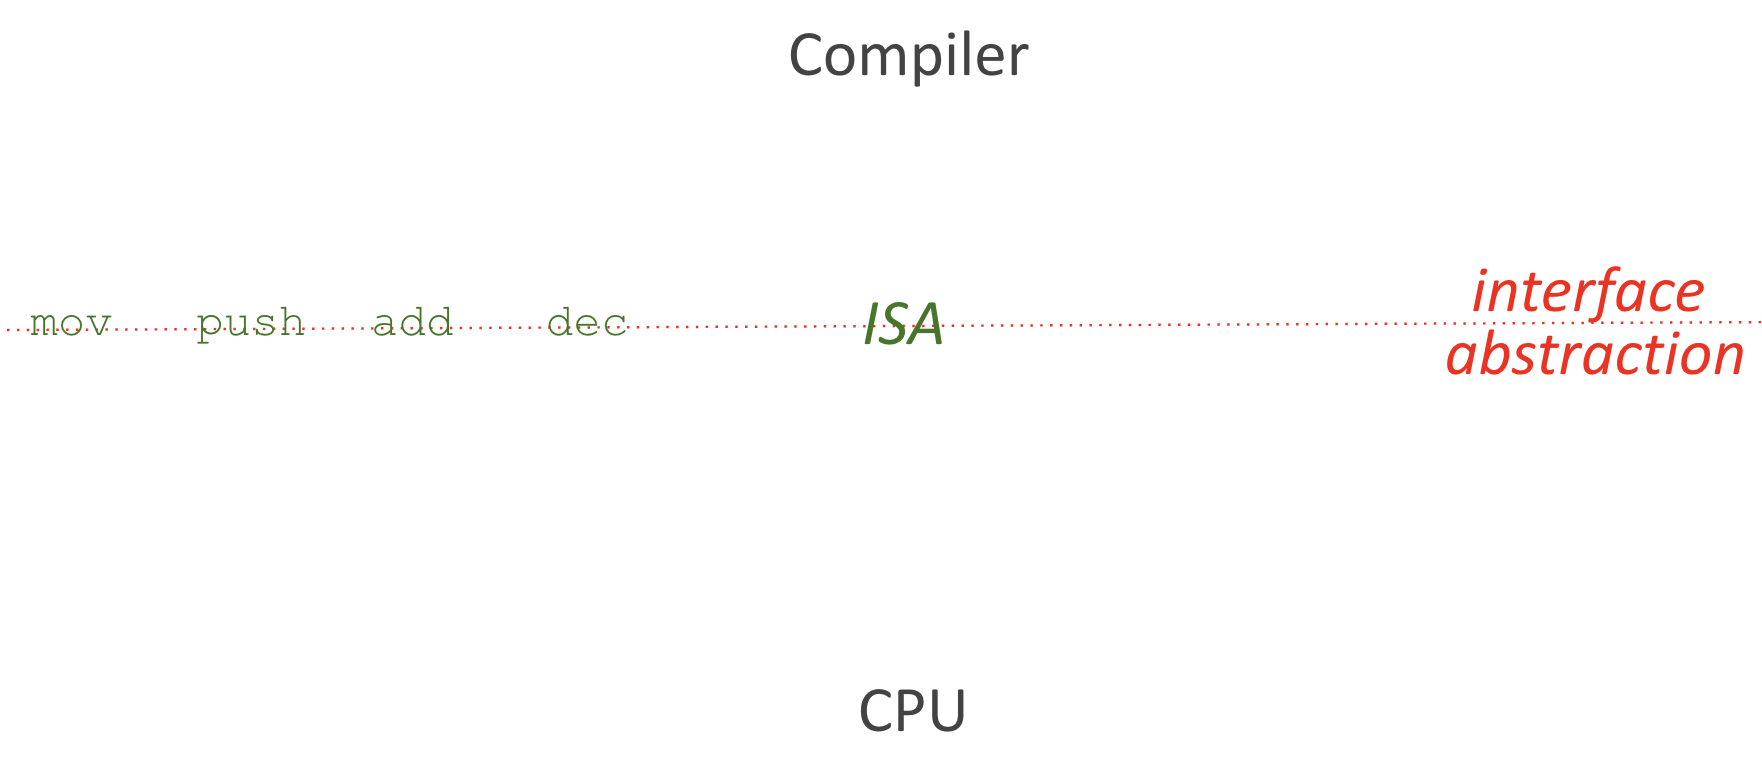
\includegraphics[width=1.25\textwidth]{chapters/L1/images/isa.png}
\end{center}
\end{minipage}\\
\vfill
\begin{definition}[Von Neumann Architecture]
The vast majority of computers today follow the \textbf{Von Neumann architecture}, which is characterized by a single main memory that holds both data and instructions.

\begin{center}
  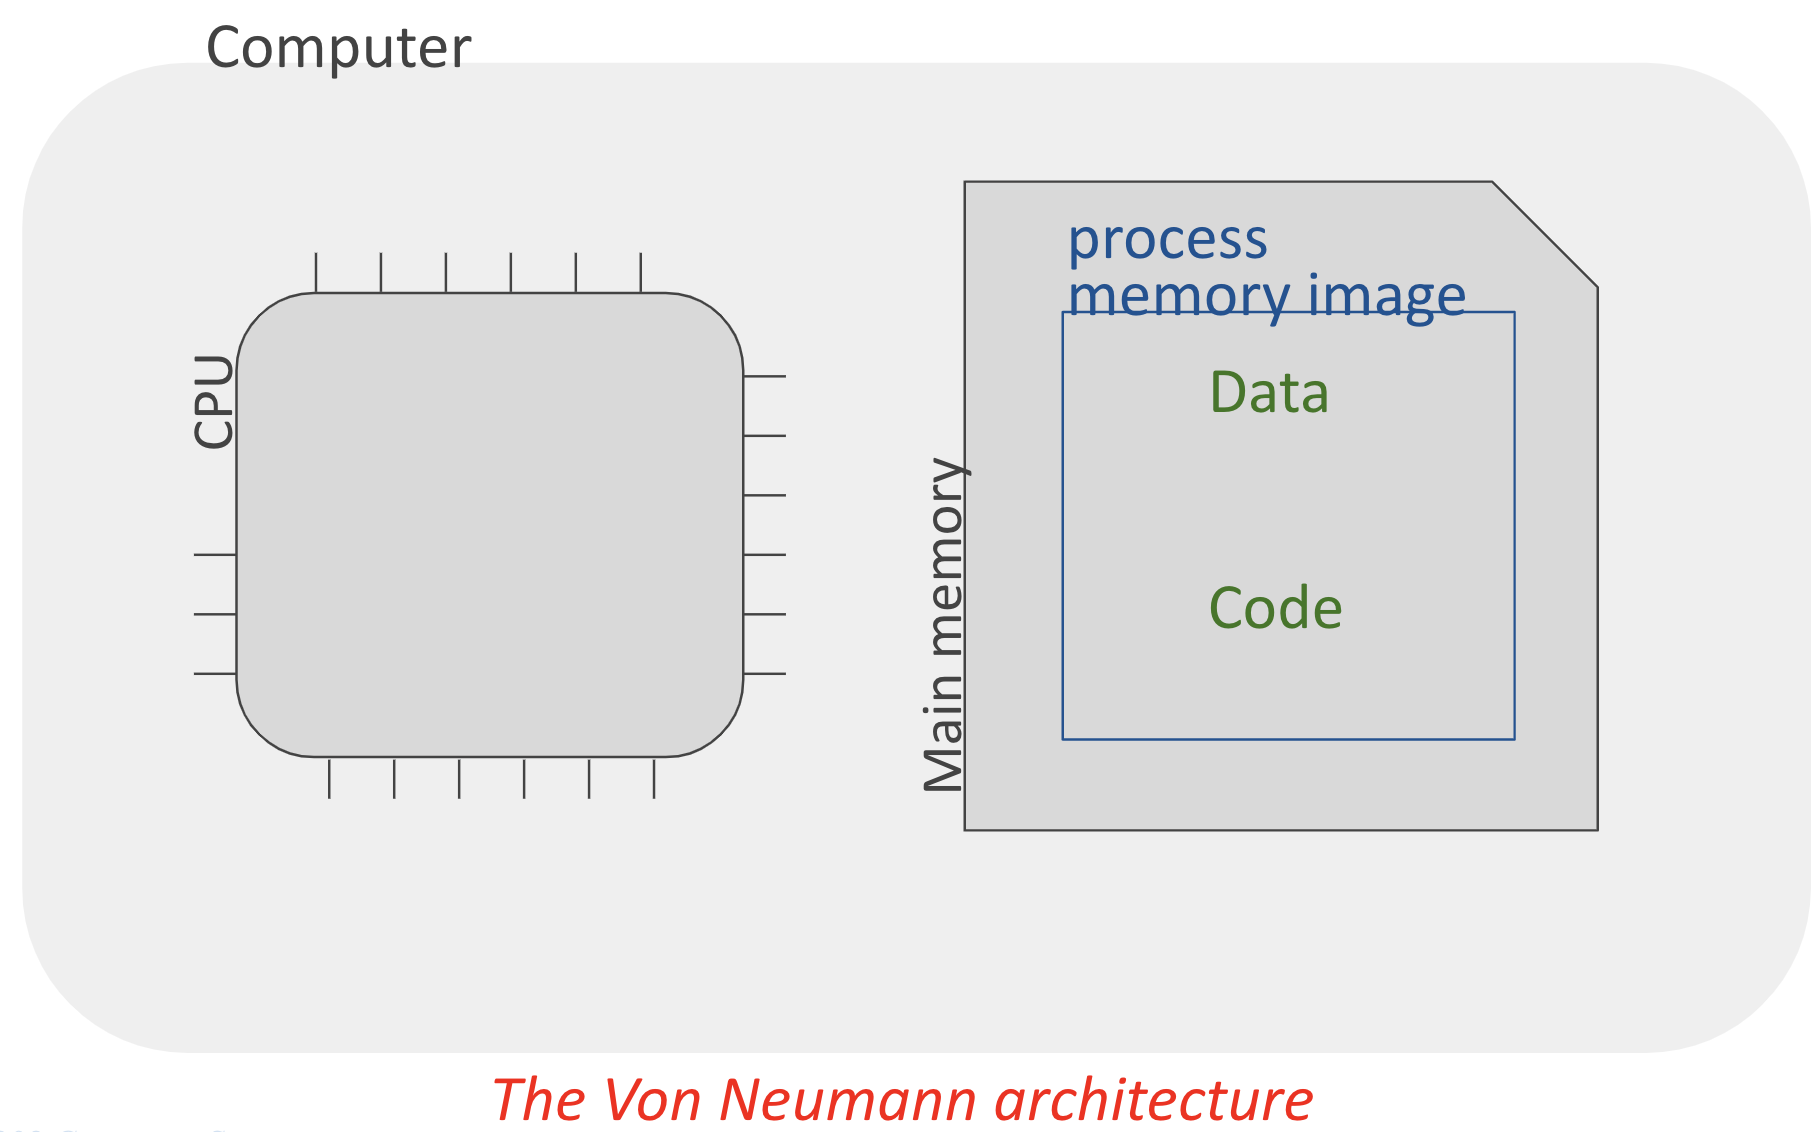
\includegraphics[width=0.55\textwidth]{chapters/L1/images/von.png}
\end{center}
\end{definition}

%%%%%%%%%%%%%%%%%%%%%%%%%%%%%%%%%%%%%%%%%%%%%%%%%%%%%%%%%%%%%%%%%%%%%%
\begin{definition}[CPU Frequency]
A CPU’s frequency indicates how many cycles it can perform in one second. For example, a 4.05~GHz CPU performs 4.05 billion cycles per second. In this context, a \textbf{cycle} is the minimum time needed for the CPU to complete an operation or for a result to become ready.\\
\vspace{0.5em}
{\textbf{Question:} What is the meaning of the Hz metric?}\\[0.5em]
\textbf{Answer:} Hertz (Hz) measures the number of cycles per second.
\vspace{0.5em}
{\textbf{Question:} In the context of a CPU, what is a cycle?}\\[0.5em]
\textbf{Answer:} A cycle is the minimum unit of time required for the CPU to produce a result from executing an instruction.
\end{definition}


%%%%%%%%%%%%%%%%%%%%%%%%%%%%%%%%%%%%%%%%%%%%%%%%%%%%%%%%%%%%%%%%%%%%%%
\section{Frequency Imbalance and CPU Caching}

Modern systems exhibit a \emph{frequency imbalance} between the CPU and main memory. While the CPU might complete an instruction in approximately 1~nsec, accessing data from DRAM typically takes 50–150~nsec. As a result, the CPU can spend a significant amount of time idle, waiting for data.

\begin{center}
  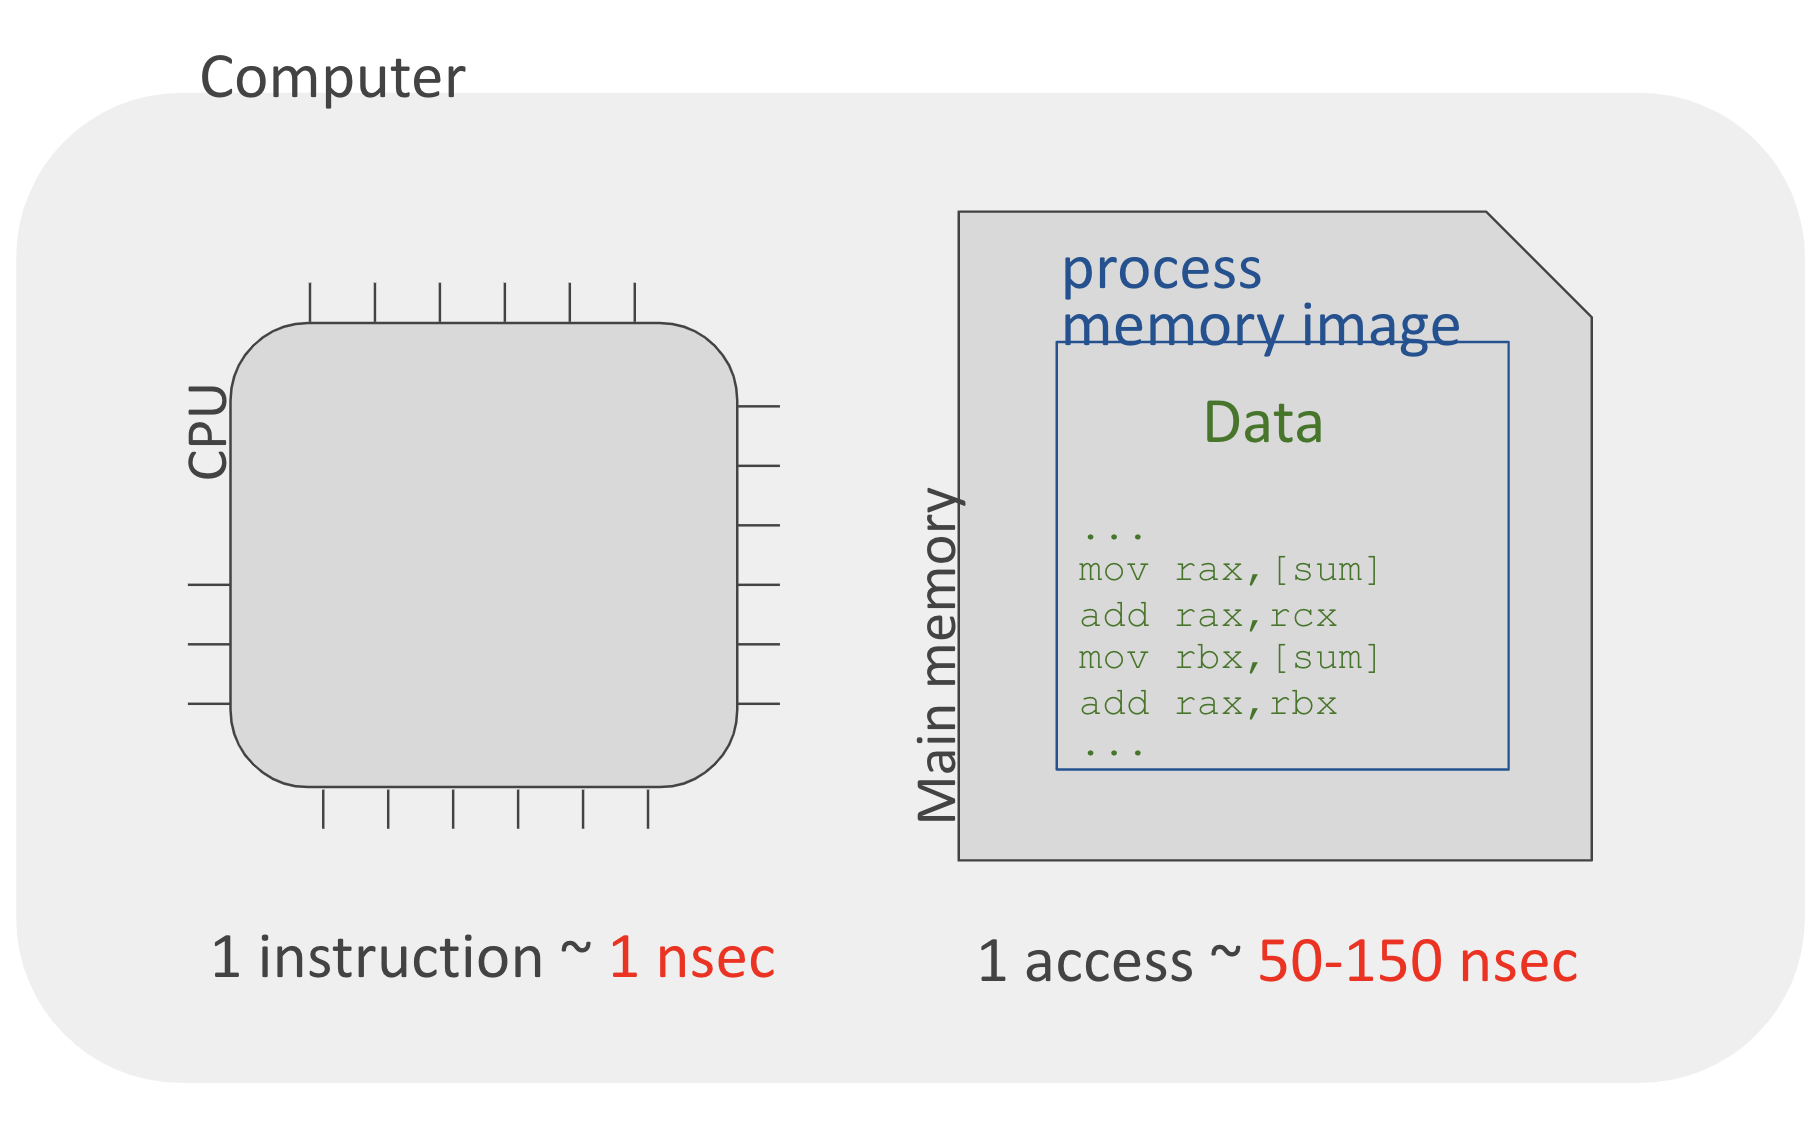
\includegraphics[width=0.65\textwidth]{chapters/L1/images/imbalance.png}
\end{center}

\vspace{0.5em}
{\textbf{Question:} How can we improve the efficiency of a system with such a frequency imbalance?}\\[0.5em]
\textbf{Answer:} We can improve efficiency by using caching. A small, fast memory (the CPU cache) stores recently accessed data so that subsequent accesses are much faster.
\newpage
\subsection{CPU Caching}
CPU caching adds a small amount of high-speed memory inside the CPU. When data is requested, the cache is checked first. If the data is already in the cache (a cache hit), the CPU retrieves it quickly. Otherwise (a cache miss), the data is fetched from the slower main memory and stored in the cache for future accesses.

\begin{center}
  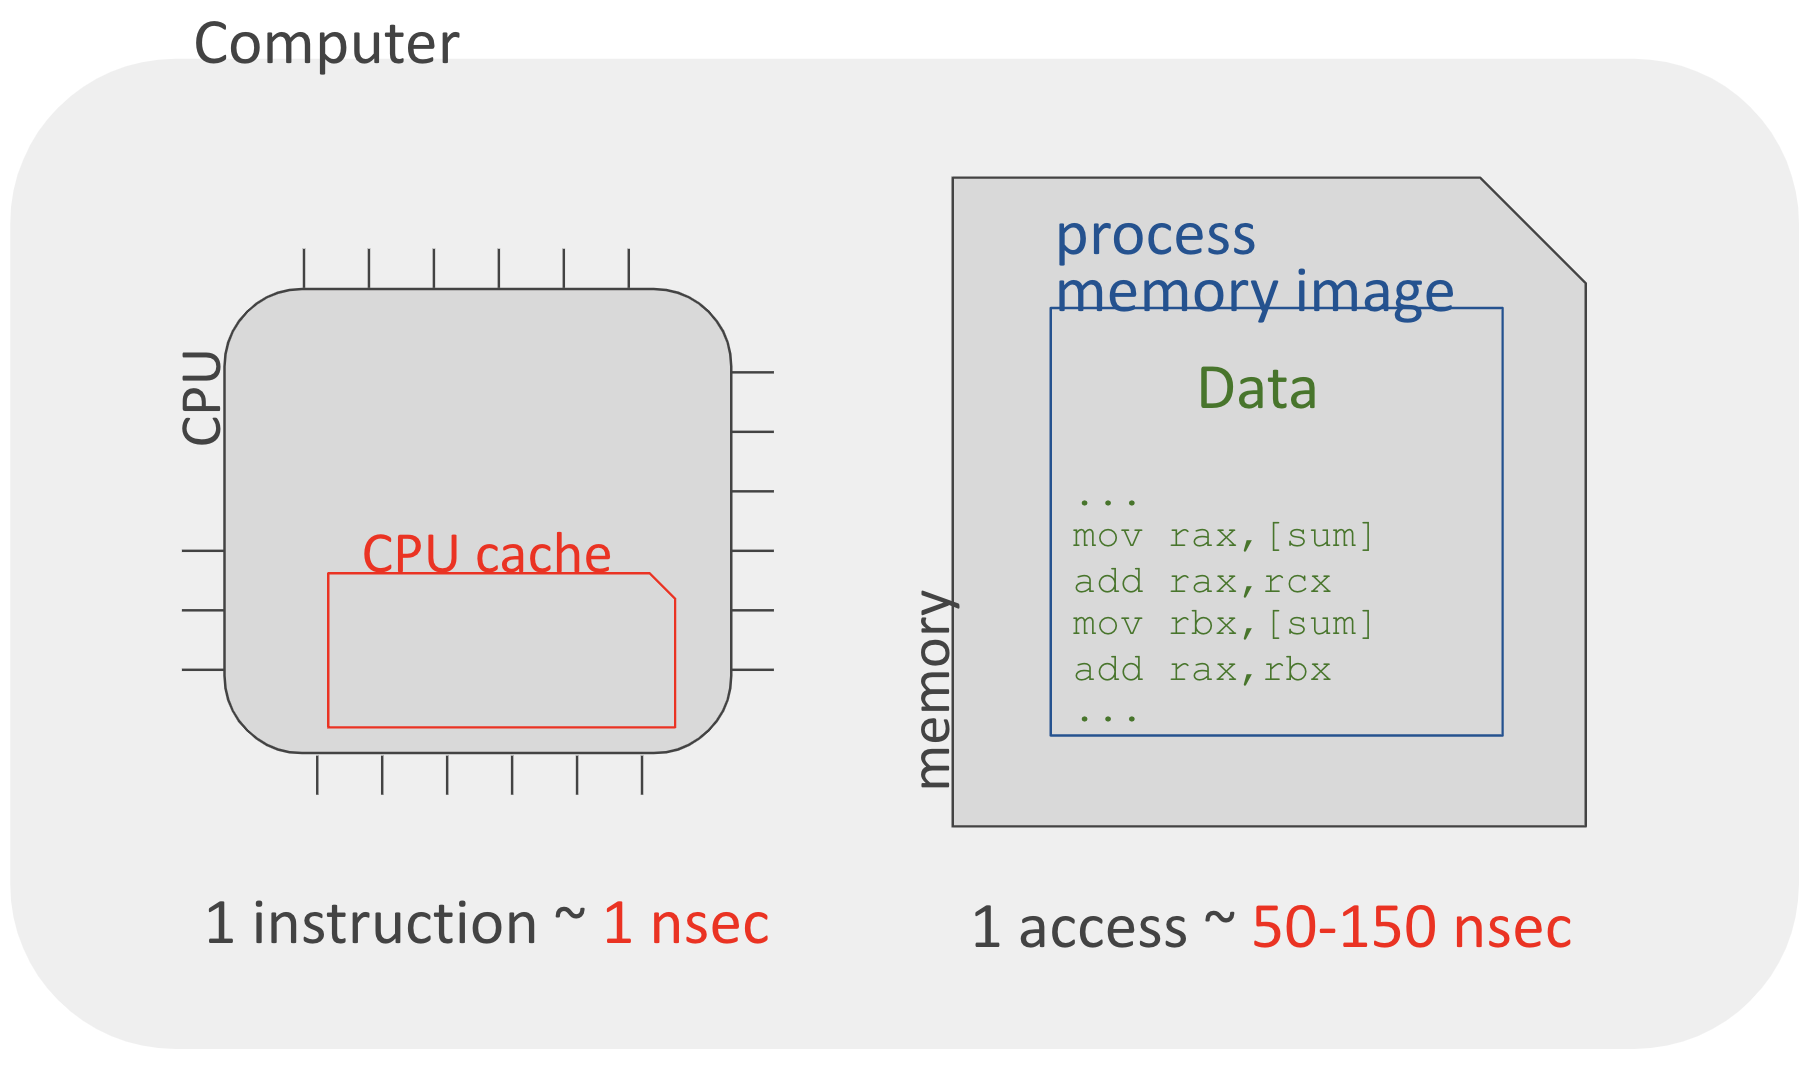
\includegraphics[width=0.65\textwidth]{chapters/L1/images/cache.png}
\end{center}

%%%%%%%%%%%%%%%%%%%%%%%%%%%%%%%%%%%%%%%%%%%%%%%%%%%%%%%%%%%%%%%%%%%%%%
\section{Memory Accesses vs. I/O}

\subsection{Memory Accesses}
When a process reads or writes data in main memory, it uses fast CPU instructions (load/store). These operations are efficient and do not interrupt the normal flow of the process.

\subsection{Back to YouTube Fetching: System Calls in Action}

Returning to our YouTube example, when the browser process calls a \texttt{send} syscall to request a video, the CPU stops executing the browser’s code and switches to executing the more privileged code in the OS. This is because accessing external resources (network or storage) requires a syscall.

\begin{center}
  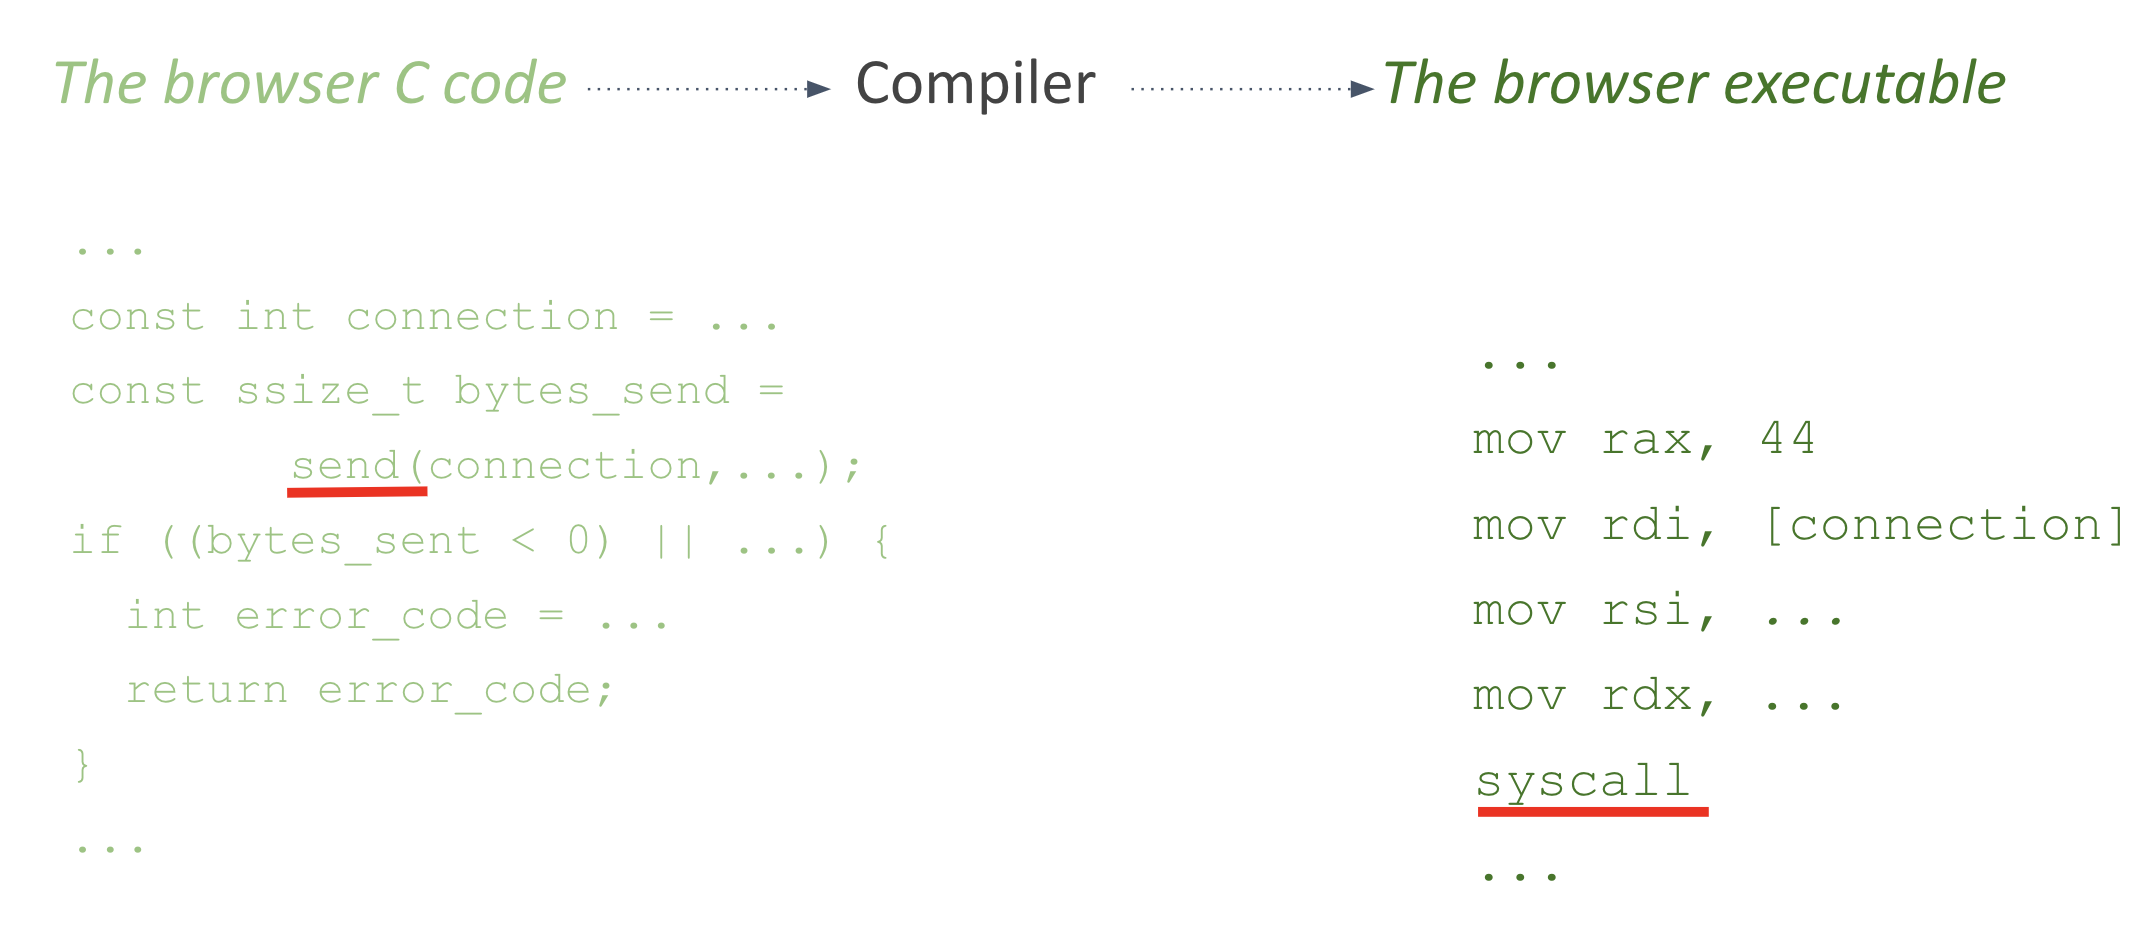
\includegraphics[width=0.85\textwidth]{chapters/L1/images/syscalls2.png}
\end{center}
\newpage
\subsection{Mixing Interfaces}
When a process makes a syscall for network communication (such as \texttt{send} or \texttt{recv}), the CPU transitions from running the process’s code to running the OS code associated with the network stack. This is an example of mixing different interfaces: the process interface (its own code) and the OS interface (syscalls).
\begin{center}
  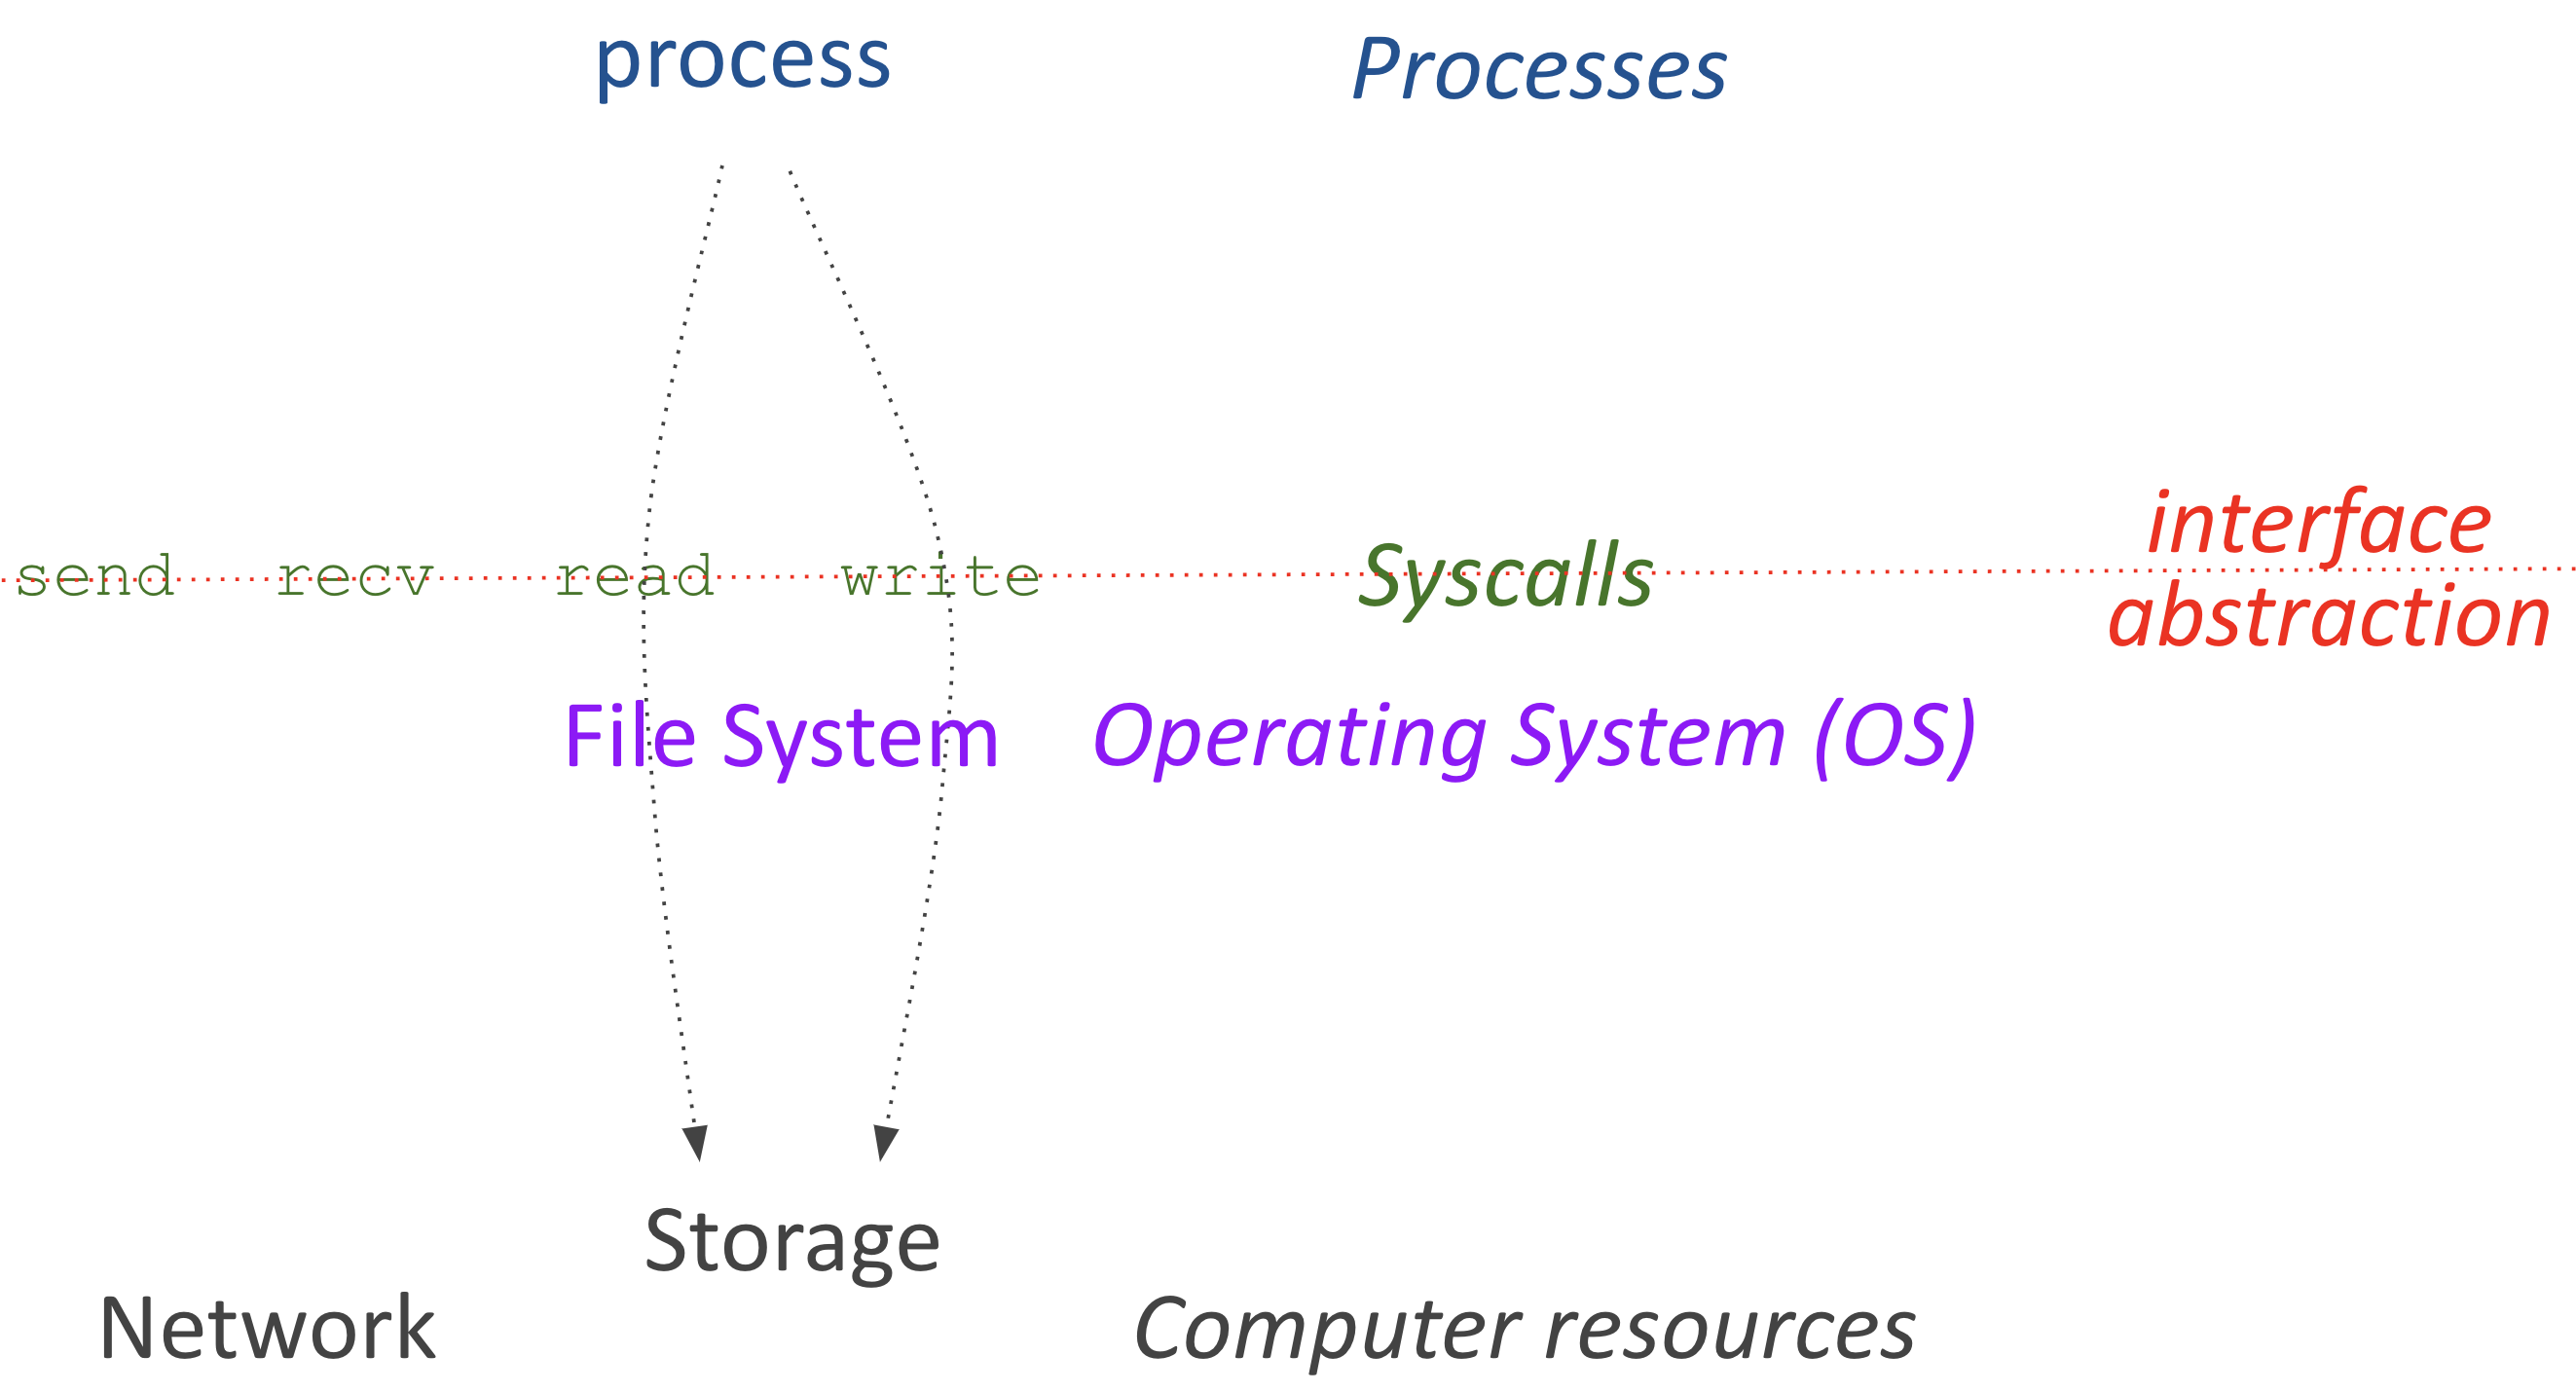
\includegraphics[width=0.65\textwidth]{chapters/L1/images/mix_int.png}
\end{center}
\vfill
\begin{definition}[Memory Access and I/O]
\textbf{Memory Access} refers to the CPU’s direct read/write operations using load/store instructions in main memory. In contrast, \textbf{I/O (Input/Output)} involves accessing external devices (such as storage or network) via system calls. I/O operations are generally more expensive because they require the CPU to switch context to execute privileged OS code.
\end{definition}
\vspace{0.5em}
\textbf{Exam Question:} How is reading from main memory different from reading from storage or the network? \\[0.5em]
\textbf{Answer:} Reading from main memory uses direct CPU instructions (load/store) and is very fast (tens to hundreds of nanoseconds), whereas reading from storage or the network requires a syscall, which interrupts the process and involves additional overhead (microseconds to milliseconds).
\vfill
\begin{definition}[I/O]
\textbf{I/O} (Input/Output) refers to operations that allow a process to access resources outside of its immediate control, such as storage devices or the network, via system calls. I/O operations are generally slower than direct memory accesses.
\end{definition}
\vspace{0.5em}
\textbf{Exam Question:} If a program does not create or manipulate any data, will executing this program require reading anything from memory?\\[0.5em]
\textbf{Answer:} Yes, executing the program will still require reading something from memory. Even if the program does not create or manipulate any data, the CPU must at least fetch the instructions of the program itself from memory

\newpage
%%%%%%%%%%%%%%%%%%%%%%%%%%%%%%%%%%%%%%%%%%%%%%%%%%%%%%%%%%%%%%%%%%%%%%
\vfill
\section{Communication Over the Internet}
Internet communication involves transferring data over a network where different latencies are encountered: \\
\begin{minipage}{0.45\textwidth}
  \begin{itemize}
    \item[-] Simple CPU instructions: \(\sim\)1~nsec.
    \item[-] Main memory accesses: tens to hundreds of nanoseconds.
    \item[-] Reading 1~KB from an SSD: tens to hundreds of microseconds.
    \item[-] Requesting data over the Internet: several to hundreds of milliseconds.
\end{itemize}
\end{minipage}
\hfill
\vline
\hfill
\begin{minipage}{0.45\textwidth}
\begin{center}
  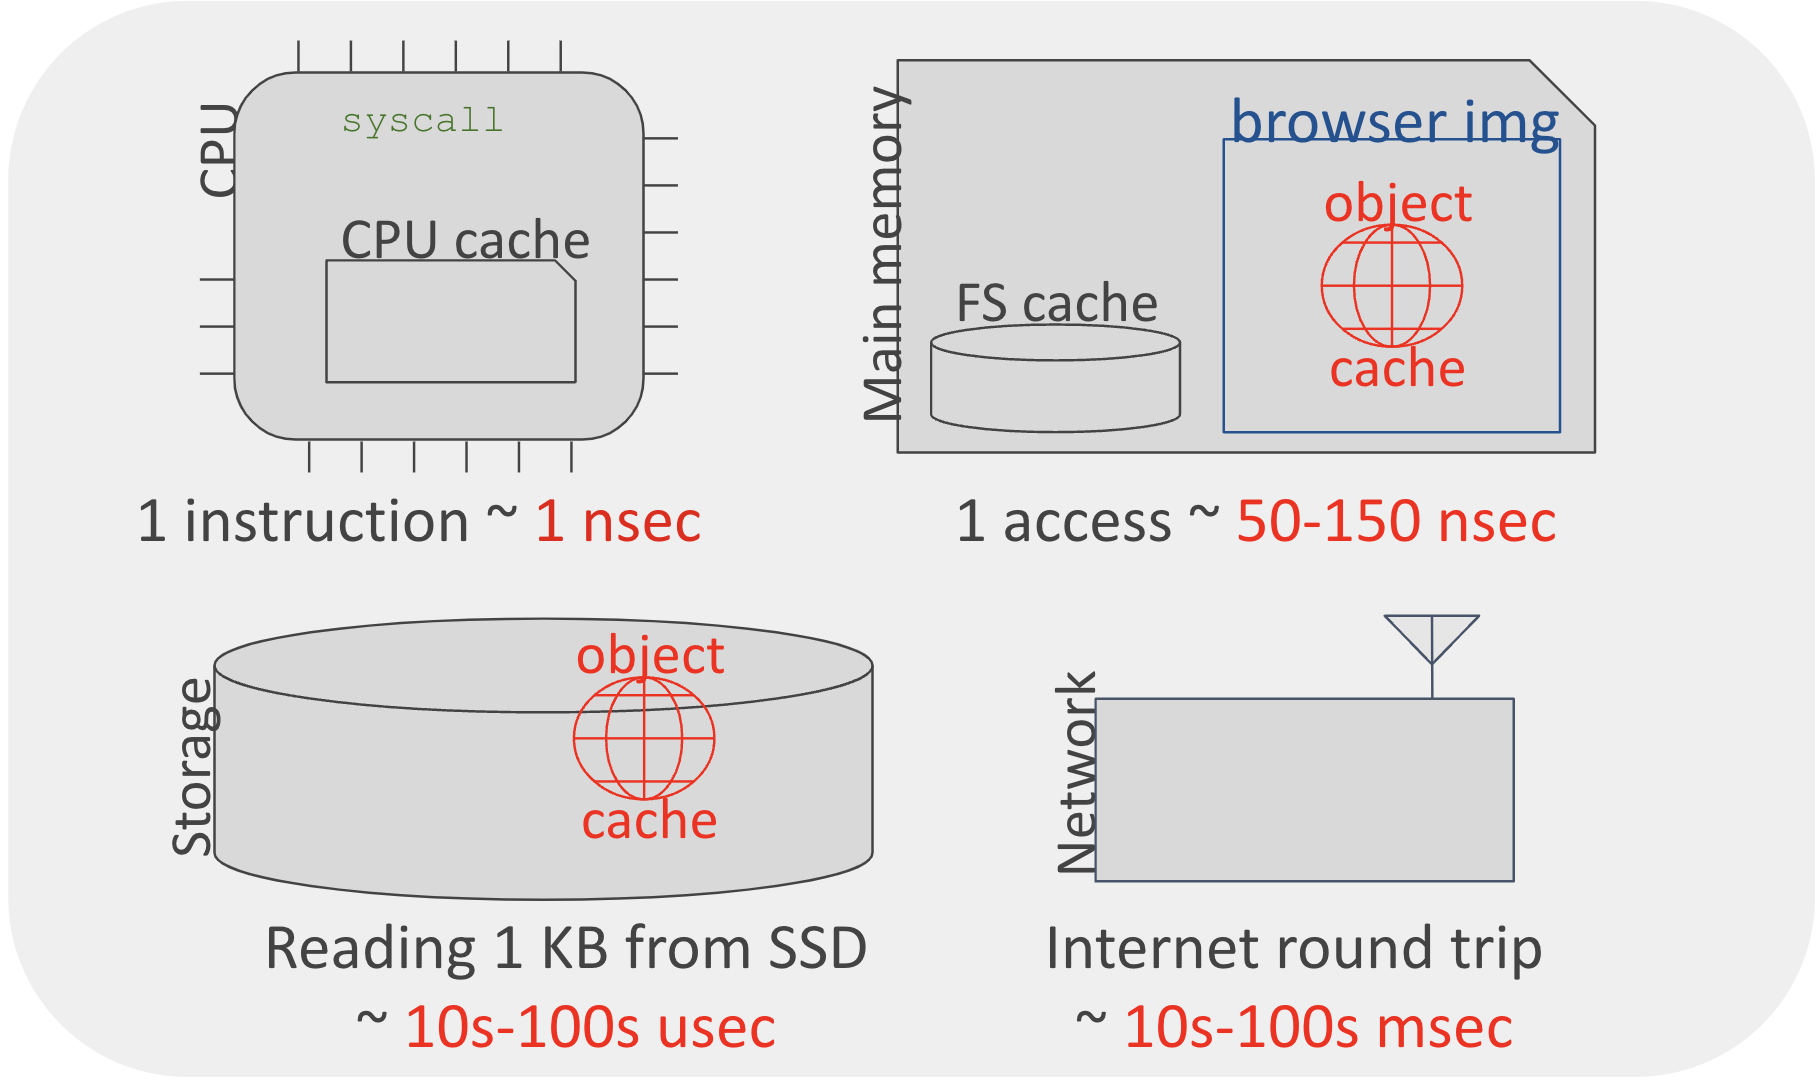
\includegraphics[width=1.15\textwidth]{chapters/L1/images/internet.png}
\end{center}
\end{minipage}\\[5px]
These delays make network communication expensive in terms of time, which is why caching is critical.
\vfill
%%%%%%%%%%%%%%%%%%%%%%%%%%%%%%%%%%%%%%%%%%%%%%%%%%%%%%%%%%%%%%%%%%%%%%
\subsection{End Systems}

The Internet is composed of \textbf{end systems}—devices that use the network for communication. These include laptops, smartphones, household appliances, connected cars, and even medical devices, as well as large cloud servers.

\begin{center}
  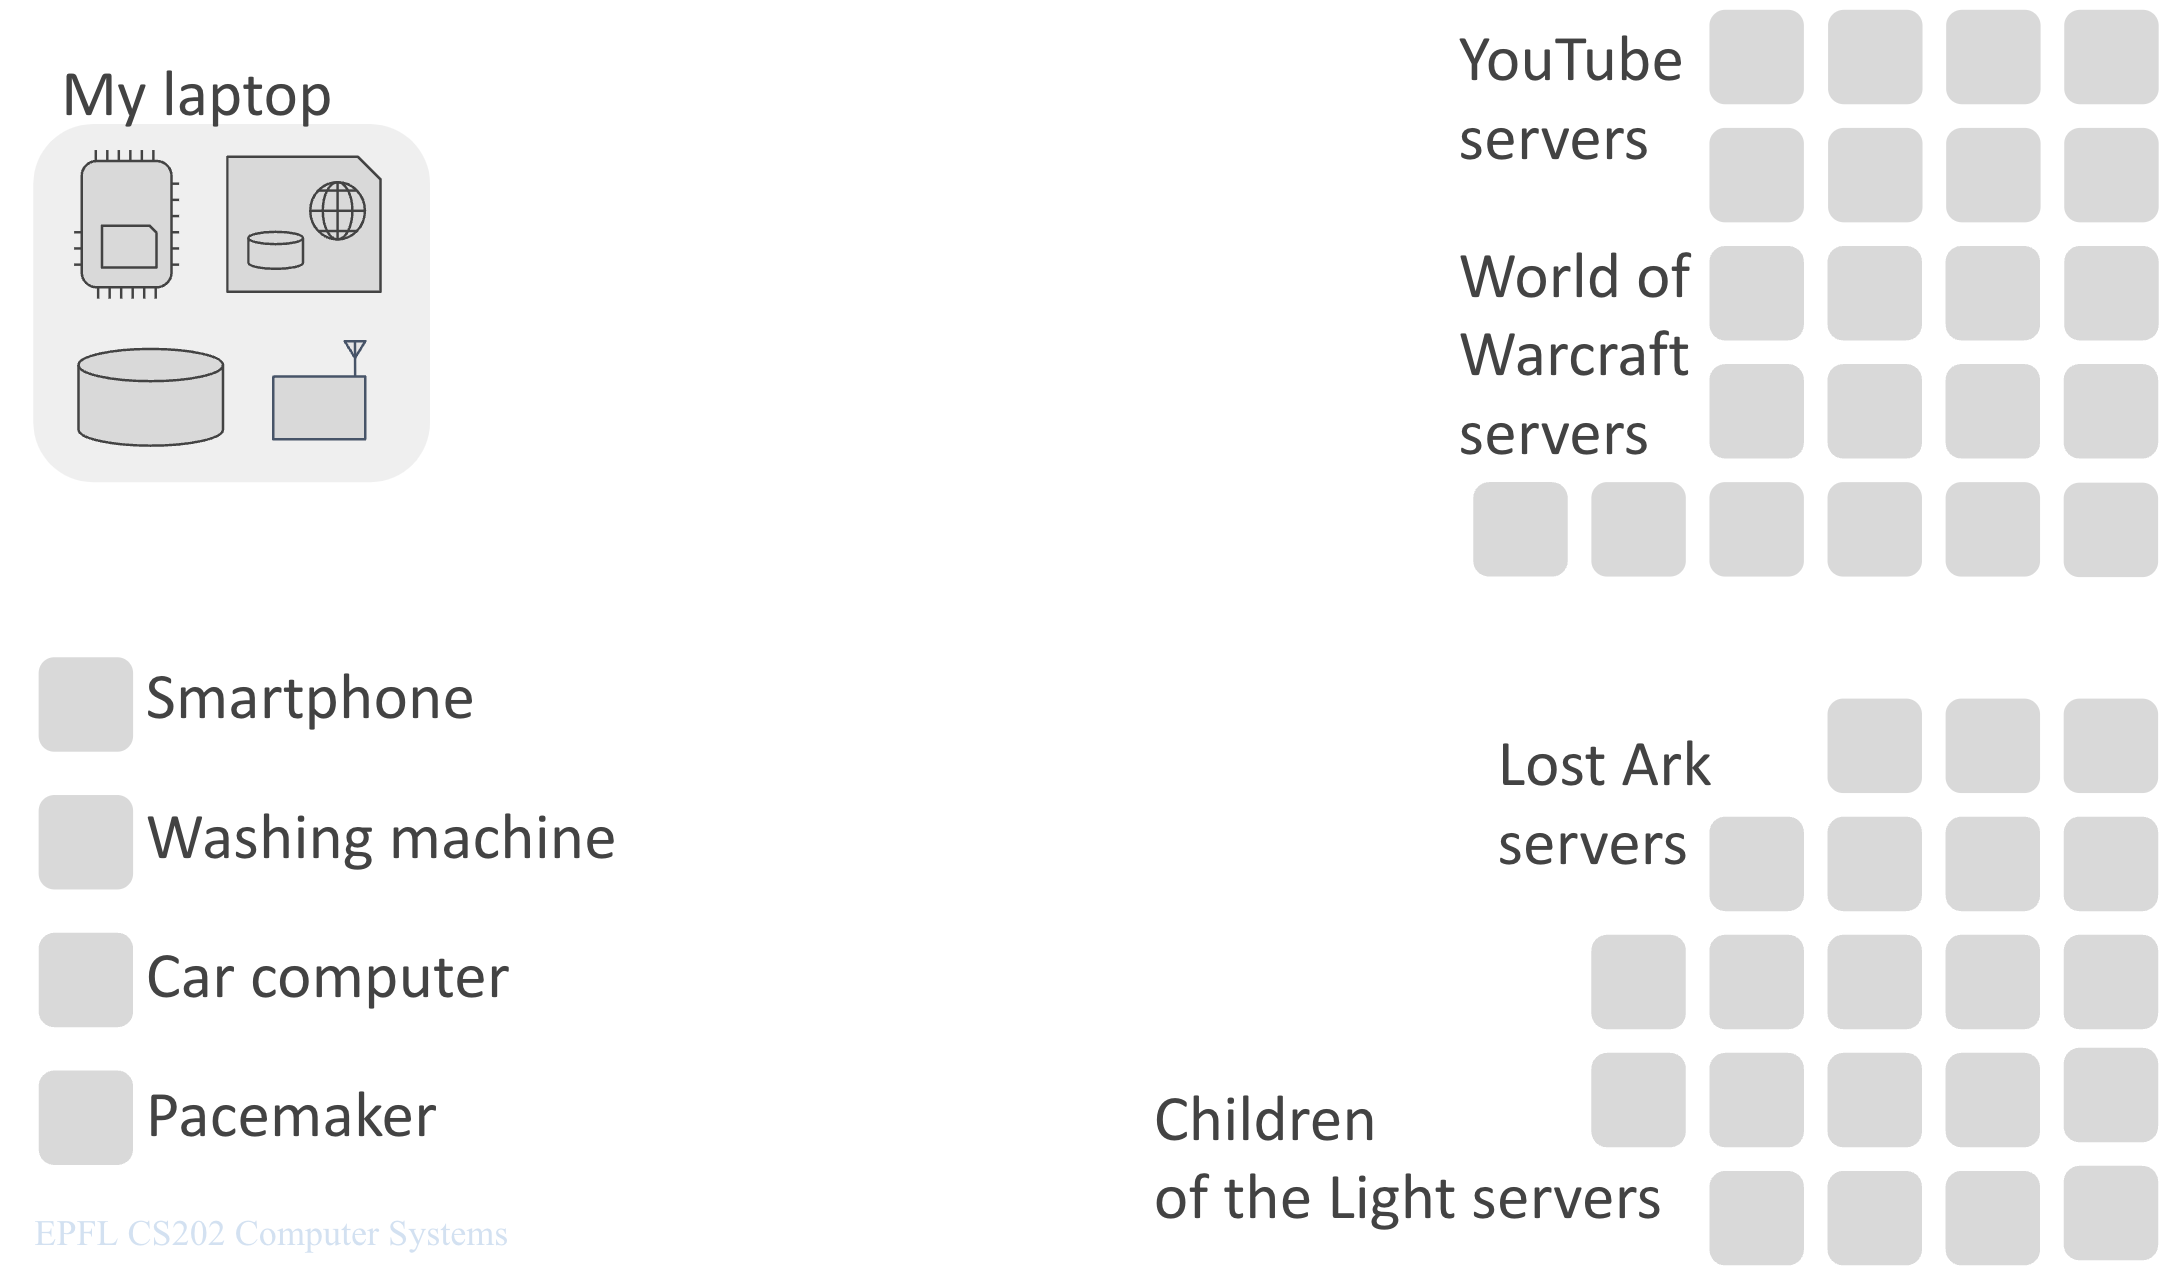
\includegraphics[width=0.65\textwidth]{chapters/L1/images/endsys.png}
\end{center}
\vfill
\newpage
%%%%%%%%%%%%%%%%%%%%%%%%%%%%%%%%%%%%%%%%%%%%%%%%%%%%%%%%%%%%%%%%%%%%%%
\subsection{Packet Switches and Network Links}

In addition to end systems, the Internet relies on:
\begin{itemize}
  \item[-] \textbf{Packet Switches}: Devices that route data between end systems.
  \item[-] \textbf{Network Links}: Physical connections that interconnect packet switches and end systems.
\end{itemize}

These components are managed by Internet Service Providers (ISPs) as well as major cloud providers.

\begin{center}
  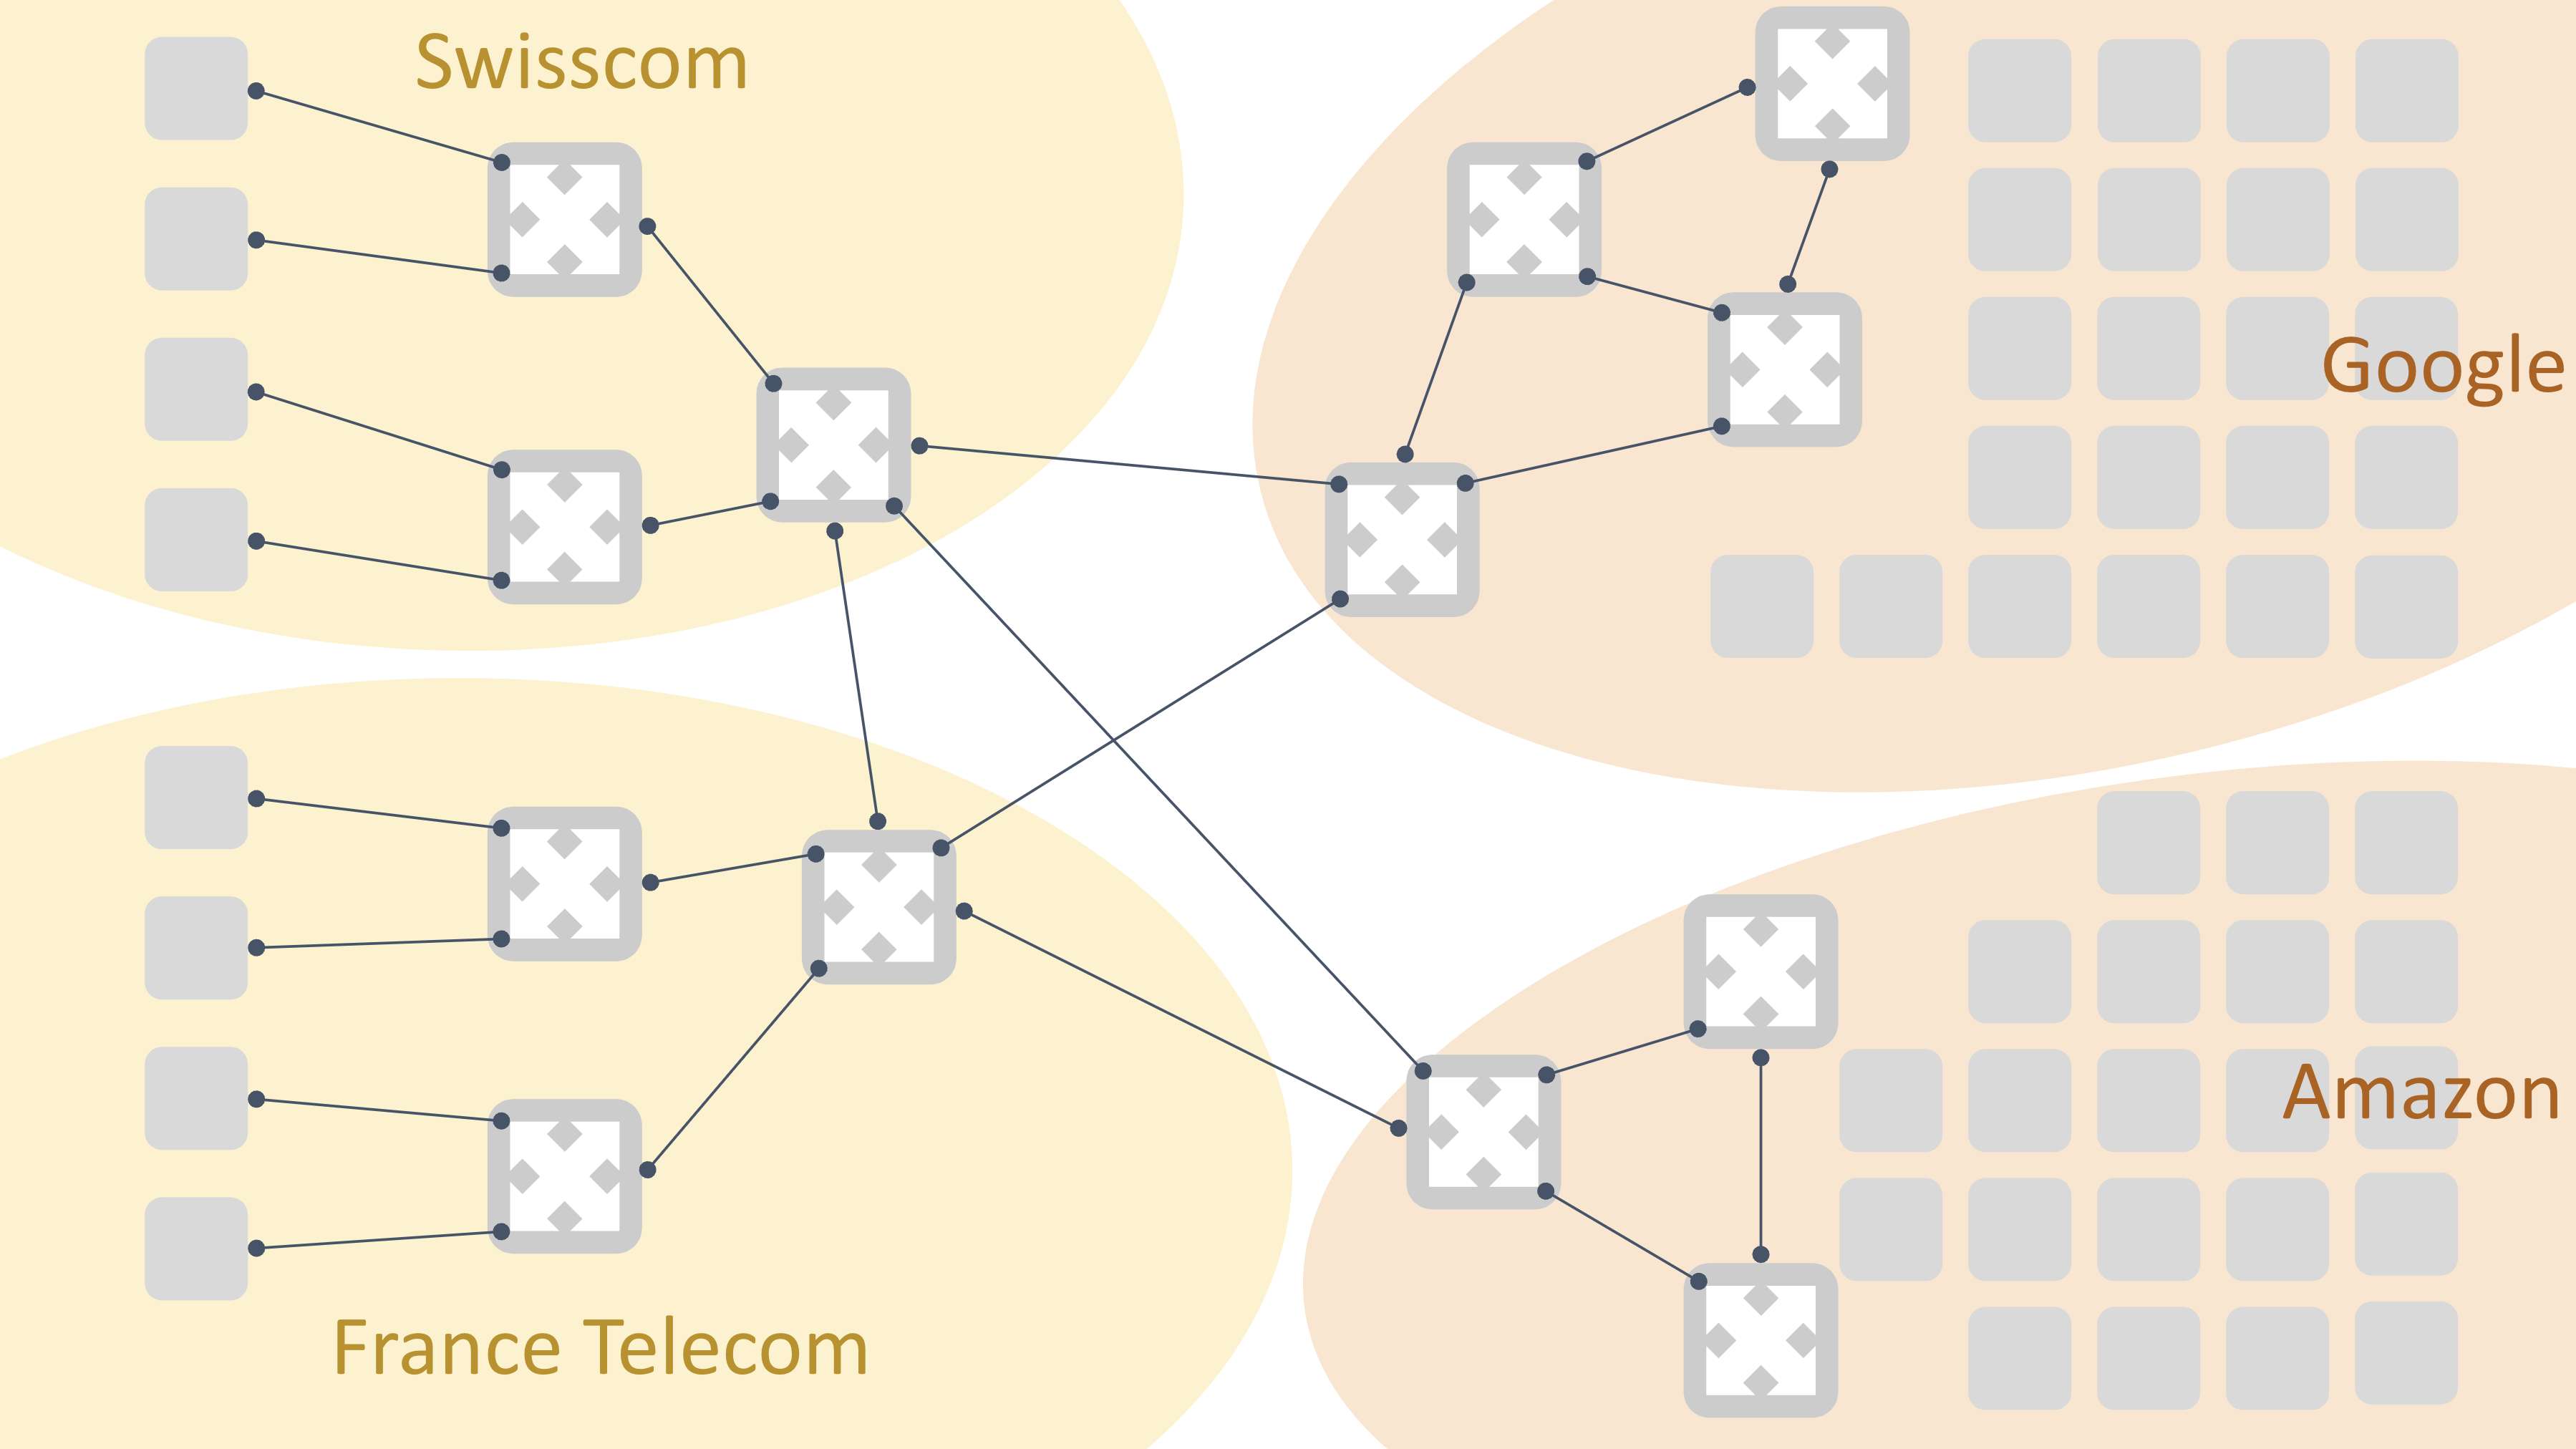
\includegraphics[width=0.65\textwidth]{chapters/L1/images/internet_schema.png}
\end{center}

%%%%%%%%%%%%%%%%%%%%%%%%%%%%%%%%%%%%%%%%%%%%%%%%%%%%%%%%%%%%%%%%%%%%%%
\subsection{Edge Caches}
To reduce the load on cloud data centers and improve user performance, large cloud providers often deploy \textbf{edge caches} within ISP networks. These caches store frequently accessed content closer to the end-users, reducing latency and network traffic.
\begin{center}
  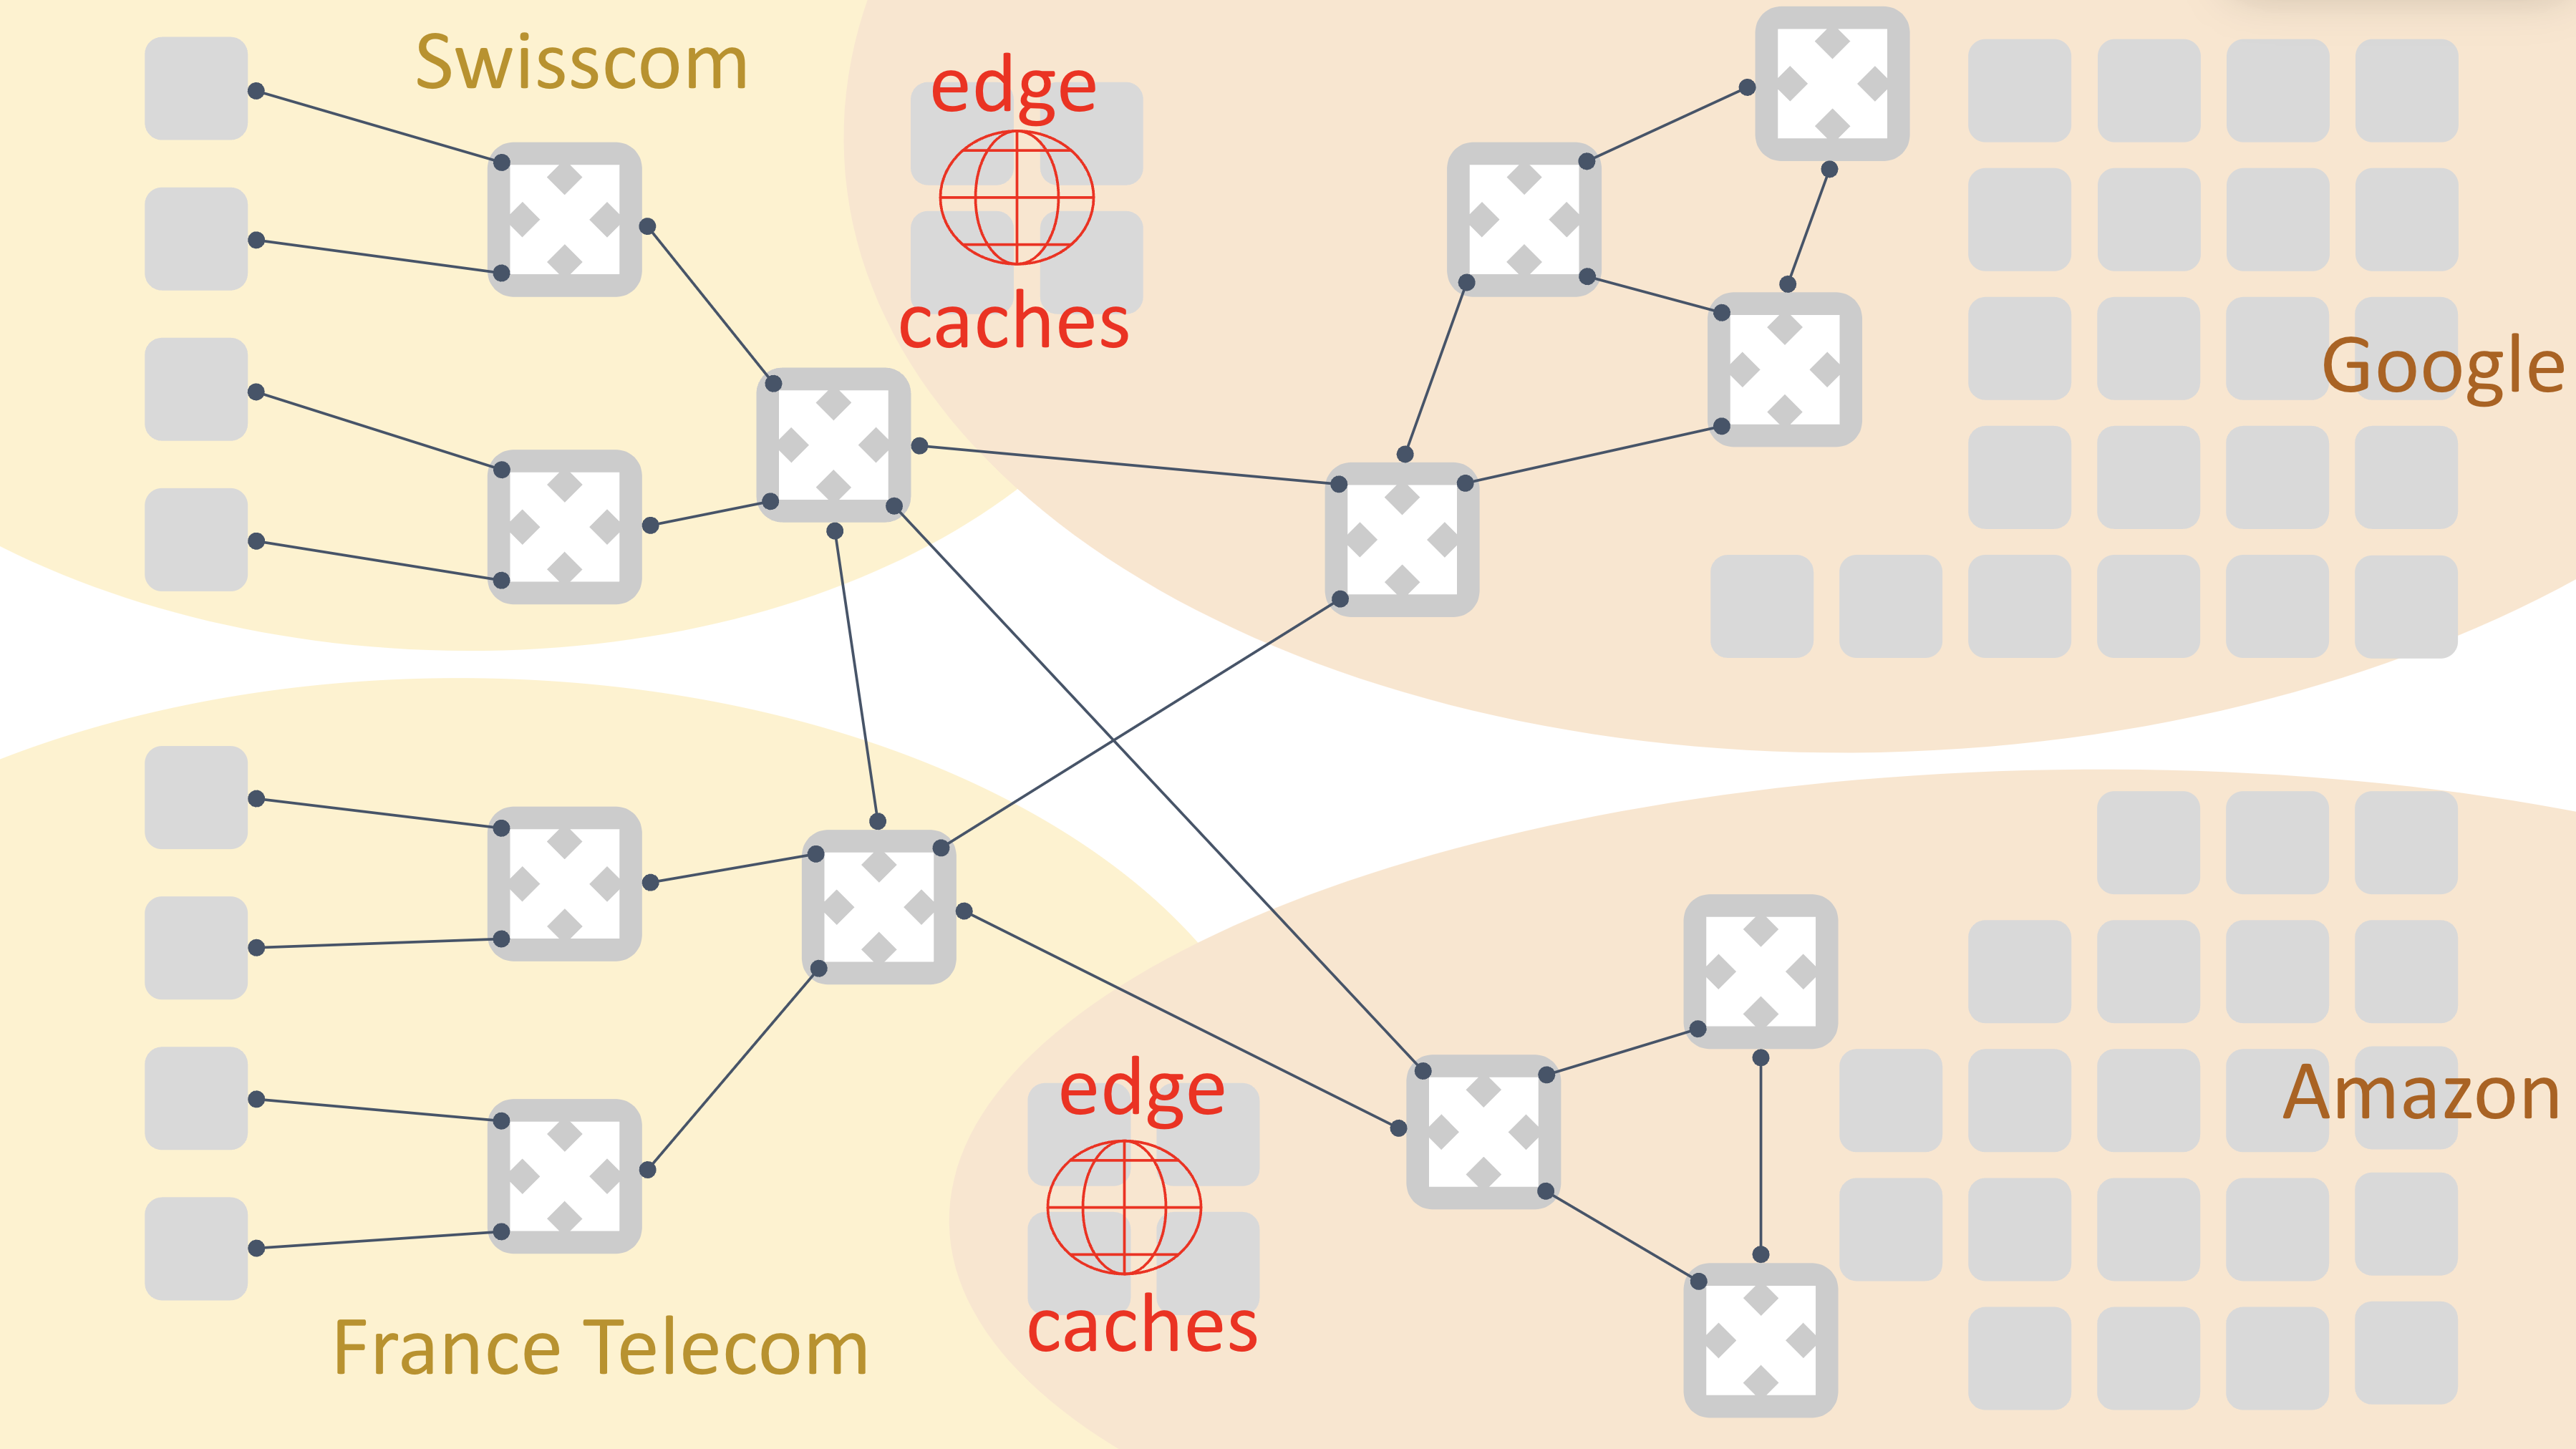
\includegraphics[width=0.65\textwidth]{chapters/L1/images/edge_caches.png}
\end{center}
%%%%%%%%%%%%%%%%%%%%%%%%%%%%%%%%%%%%%%%%%%%%%%%%%%%%%%%%%%%%%%%%%%%%%%
\section{Summary}
In this lecture, we traced the journey of a YouTube video and introduced several fundamental concepts:
\begin{itemize}
  \item \textbf{Programs, Processes, and Threads:} Programs stored on disk become processes (and threads) when executed.
  \item \textbf{Distributed Applications:} Different processes communicate over networks using well-defined communication protocols.
  \item \textbf{Interfaces and Abstractions:} System calls, APIs, and caching abstract the complexity of hardware resources.
  \item \textbf{The Operating System:} Acts as an intermediary between processes and hardware resources.
  \item \textbf{Performance Considerations:} Frequency imbalances between the CPU and memory are mitigated by caching at various levels (CPU cache, file system cache, object caches).
\end{itemize}

\begin{center}
  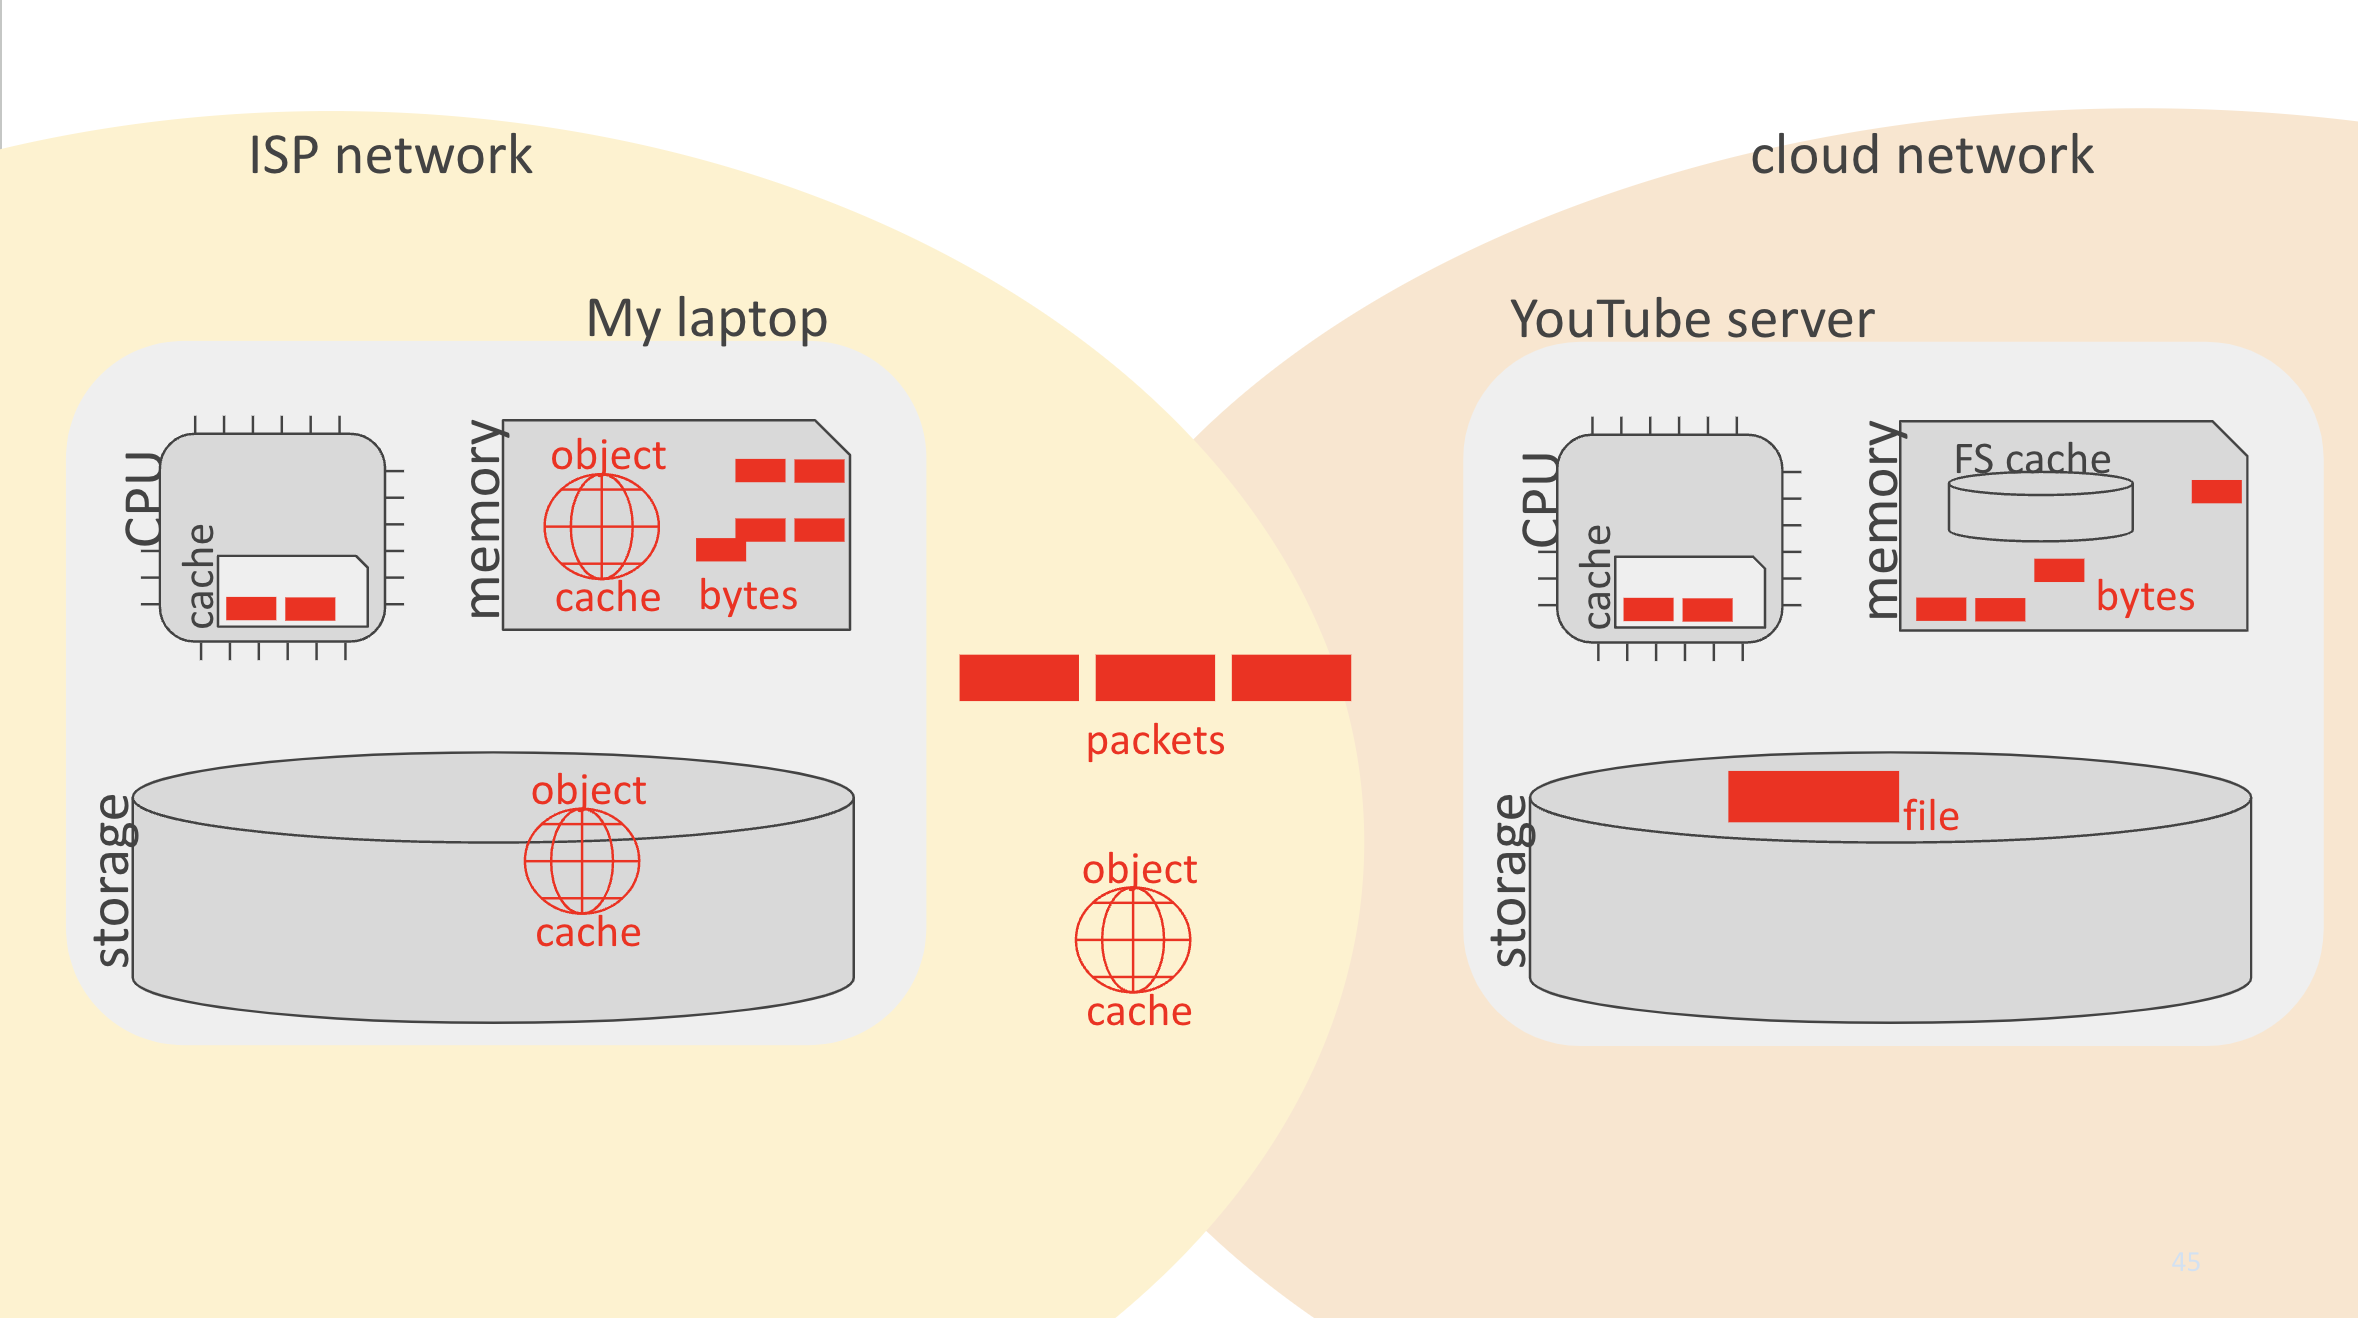
\includegraphics[width=0.65\textwidth]{chapters/L1/images/conclusion_youtube.png}
\end{center}

\end{document}
